
%% bare_jrnl.tex
%% V1.3
%% 2007/01/11
%% by Michael Shell
%% see http://www.michaelshell.org/
%% for current contact information.
%%
%% This is a skeleton file demonstrating the use of IEEEtran.cls
%% (requires IEEEtran.cls version 1.7 or later) with an IEEE journal paper.
%%
%% Support sites:
%% http://www.michaelshell.org/tex/ieeetran/
%% http://www.ctan.org/tex-archive/macros/latex/contrib/IEEEtran/
%% and
%% http://www.ieee.org/



% *** Authors should verify (and, if needed, correct) their LaTeX system  ***
% *** with the testflow diagnostic prior to trusting their LaTeX platform ***
% *** with production work. IEEE's font choices can trigger bugs that do  ***
% *** not appear when using other class files.                            ***
% The testflow support page is at:
% http://www.michaelshell.org/tex/testflow/


%%*************************************************************************
%% Legal Notice:
%% This code is offered as-is without any warranty either expressed or
%% implied; without even the implied warranty of MERCHANTABILITY or
%% FITNESS FOR A PARTICULAR PURPOSE!
%% User assumes all risk.
%% In no event shall IEEE or any contributor to this code be liable for
%% any damages or losses, including, but not limited to, incidental,
%% consequential, or any other damages, resulting from the use or misuse
%% of any information contained here.
%%
%% All comments are the opinions of their respective authors and are not
%% necessarily endorsed by the IEEE.
%%
%% This work is distributed under the LaTeX Project Public License (LPPL)
%% ( http://www.latex-project.org/ ) version 1.3, and may be freely used,
%% distributed and modified. A copy of the LPPL, version 1.3, is included
%% in the base LaTeX documentation of all distributions of LaTeX released
%% 2003/12/01 or later.
%% Retain all contribution notices and credits.
%% ** Modified files should be clearly indicated as such, including  **
%% ** renaming them and changing author support contact information. **
%%
%% File list of work: IEEEtran.cls, IEEEtran_HOWTO.pdf, bare_adv.tex,
%%                    bare_conf.tex, bare_jrnl.tex, bare_jrnl_compsoc.tex
%%*************************************************************************

% Note that the a4paper option is mainly intended so that authors in
% countries using A4 can easily print to A4 and see how their papers will
% look in print - the typesetting of the document will not typically be
% affected with changes in paper size (but the bottom and side margins will).
% Use the testflow package mentioned above to verify correct handling of
% both paper sizes by the user's LaTeX system.
%
% Also note that the "draftcls" or "draftclsnofoot", not "draft", option
% should be used if it is desired that the figures are to be displayed in
% draft mode.
%
\documentclass[journal]{IEEEtran}
%
% If IEEEtran.cls has not been installed into the LaTeX system files,
% manually specify the path to it like:
% \documentclass[journal]{../sty/IEEEtran}





% Some very useful LaTeX packages include:
% (uncomment the ones you want to load)


% *** MISC UTILITY PACKAGES ***
%
%\usepackage{ifpdf}
% Heiko Oberdiek's ifpdf.sty is very useful if you need conditional
% compilation based on whether the output is pdf or dvi.
% usage:
% \ifpdf
%   % pdf code
% \else
%   % dvi code
% \fi
% The latest version of ifpdf.sty can be obtained from:
% http://www.ctan.org/tex-archive/macros/latex/contrib/oberdiek/
% Also, note that IEEEtran.cls V1.7 and later provides a builtin
% \ifCLASSINFOpdf conditional that works the same way.
% When switching from latex to pdflatex and vice-versa, the compiler may
% have to be run twice to clear warning/error messages.






% *** CITATION PACKAGES ***
%
\usepackage{cite}
% cite.sty was written by Donald Arseneau
% V1.6 and later of IEEEtran pre-defines the format of the cite.sty package
% \cite{} output to follow that of IEEE. Loading the cite package will
% result in citation numbers being automatically sorted and properly
% "compressed/ranged". e.g., [1], [9], [2], [7], [5], [6] without using
% cite.sty will become [1], [2], [5]--[7], [9] using cite.sty. cite.sty's
% \cite will automatically add leading space, if needed. Use cite.sty's
% noadjust option (cite.sty V3.8 and later) if you want to turn this off.
% cite.sty is already installed on most LaTeX systems. Be sure and use
% version 4.0 (2003-05-27) and later if using hyperref.sty. cite.sty does
% not currently provide for hyperlinked citations.
% The latest version can be obtained at:
% http://www.ctan.org/tex-archive/macros/latex/contrib/cite/
% The documentation is contained in the cite.sty file itself.






% *** GRAPHICS RELATED PACKAGES ***
%
\ifCLASSINFOpdf
   \usepackage[pdftex]{graphicx}
  % declare the path(s) where your graphic files are
  % \graphicspath{{../pdf/}{../jpeg/}}
  % and their extensions so you won't have to specify these with
  % every instance of \includegraphics
  % \DeclareGraphicsExtensions{.pdf,.jpeg,.png}
\else
  % or other class option (dvipsone, dvipdf, if not using dvips). graphicx
  % will default to the driver specified in the system graphics.cfg if no
  % driver is specified.
   \usepackage[dvips]{graphicx}
  % declare the path(s) where your graphic files are
  % \graphicspath{{../eps/}}
  % and their extensions so you won't have to specify these with
  % every instance of \includegraphics
  % \DeclareGraphicsExtensions{.eps}
\fi
% graphicx was written by David Carlisle and Sebastian Rahtz. It is
% required if you want graphics, photos, etc. graphicx.sty is already
% installed on most LaTeX systems. The latest version and documentation can
% be obtained at:
% http://www.ctan.org/tex-archive/macros/latex/required/graphics/
% Another good source of documentation is "Using Imported Graphics in
% LaTeX2e" by Keith Reckdahl which can be found as epslatex.ps or
% epslatex.pdf at: http://www.ctan.org/tex-archive/info/
%
% latex, and pdflatex in dvi mode, support graphics in encapsulated
% postscript (.eps) format. pdflatex in pdf mode supports graphics
% in .pdf, .jpeg, .png and .mps (metapost) formats. Users should ensure
% that all non-photo figures use a vector format (.eps, .pdf, .mps) and
% not a bitmapped formats (.jpeg, .png). IEEE frowns on bitmapped formats
% which can result in "jaggedy"/blurry rendering of lines and letters as
% well as large increases in file sizes.
%
% You can find documentation about the pdfTeX application at:
% http://www.tug.org/applications/pdftex





% *** MATH PACKAGES ***
%
\usepackage[cmex10]{amsmath}
\usepackage{amssymb}
% A popular package from the American Mathematical Society that provides
% many useful and powerful commands for dealing with mathematics. If using
% it, be sure to load this package with the cmex10 option to ensure that
% only type 1 fonts will utilized at all point sizes. Without this option,
% it is possible that some math symbols, particularly those within
% footnotes, will be rendered in bitmap form which will result in a
% document that can not be IEEE Xplore compliant!
%
% Also, note that the amsmath package sets \interdisplaylinepenalty to 10000
% thus preventing page breaks from occurring within multiline equations. Use:
%\interdisplaylinepenalty=2500
% after loading amsmath to restore such page breaks as IEEEtran.cls normally
% does. amsmath.sty is already installed on most LaTeX systems. The latest
% version and documentation can be obtained at:
% http://www.ctan.org/tex-archive/macros/latex/required/amslatex/math/





% *** SPECIALIZED LIST PACKAGES ***
%
%\usepackage{algorithmic}
% algorithmic.sty was written by Peter Williams and Rogerio Brito.
% This package provides an algorithmic environment fo describing algorithms.
% You can use the algorithmic environment in-text or within a figure
% environment to provide for a floating algorithm. Do NOT use the algorithm
% floating environment provided by algorithm.sty (by the same authors) or
% algorithm2e.sty (by Christophe Fiorio) as IEEE does not use dedicated
% algorithm float types and packages that provide these will not provide
% correct IEEE style captions. The latest version and documentation of
% algorithmic.sty can be obtained at:
% http://www.ctan.org/tex-archive/macros/latex/contrib/algorithms/
% There is also a support site at:
% http://algorithms.berlios.de/index.html
% Also of interest may be the (relatively newer and more customizable)
% algorithmicx.sty package by Szasz Janos:
% http://www.ctan.org/tex-archive/macros/latex/contrib/algorithmicx/




% *** ALIGNMENT PACKAGES ***
%
%\usepackage{array}
% Frank Mittelbach's and David Carlisle's array.sty patches and improves
% the standard LaTeX2e array and tabular environments to provide better
% appearance and additional user controls. As the default LaTeX2e table
% generation code is lacking to the point of almost being broken with
% respect to the quality of the end results, all users are strongly
% advised to use an enhanced (at the very least that provided by array.sty)
% set of table tools. array.sty is already installed on most systems. The
% latest version and documentation can be obtained at:
% http://www.ctan.org/tex-archive/macros/latex/required/tools/


%\usepackage{mdwmath}
%\usepackage{mdwtab}
% Also highly recommended is Mark Wooding's extremely powerful MDW tools,
% especially mdwmath.sty and mdwtab.sty which are used to format equations
% and tables, respectively. The MDWtools set is already installed on most
% LaTeX systems. The lastest version and documentation is available at:
% http://www.ctan.org/tex-archive/macros/latex/contrib/mdwtools/


% IEEEtran contains the IEEEeqnarray family of commands that can be used to
% generate multiline equations as well as matrices, tables, etc., of high
% quality.


%\usepackage{eqparbox}
% Also of notable interest is Scott Pakin's eqparbox package for creating
% (automatically sized) equal width boxes - aka "natural width parboxes".
% Available at:
% http://www.ctan.org/tex-archive/macros/latex/contrib/eqparbox/





% *** SUBFIGURE PACKAGES ***
%\usepackage[tight,footnotesize]{subfigure}
% subfigure.sty was written by Steven Douglas Cochran. This package makes it
% easy to put subfigures in your figures. e.g., "Figure 1a and 1b". For IEEE
% work, it is a good idea to load it with the tight package option to reduce
% the amount of white space around the subfigures. subfigure.sty is already
% installed on most LaTeX systems. The latest version and documentation can
% be obtained at:
% http://www.ctan.org/tex-archive/obsolete/macros/latex/contrib/subfigure/
% subfigure.sty has been superceeded by subfig.sty.



%\usepackage[caption=false]{caption}
%\usepackage[font=footnotesize]{subfig}
% subfig.sty, also written by Steven Douglas Cochran, is the modern
% replacement for subfigure.sty. However, subfig.sty requires and
% automatically loads Axel Sommerfeldt's caption.sty which will override
% IEEEtran.cls handling of captions and this will result in nonIEEE style
% figure/table captions. To prevent this problem, be sure and preload
% caption.sty with its "caption=false" package option. This is will preserve
% IEEEtran.cls handing of captions. Version 1.3 (2005/06/28) and later
% (recommended due to many improvements over 1.2) of subfig.sty supports
% the caption=false option directly:
%\usepackage[caption=false,font=footnotesize]{subfig}
%
% The latest version and documentation can be obtained at:
% http://www.ctan.org/tex-archive/macros/latex/contrib/subfig/
% The latest version and documentation of caption.sty can be obtained at:
% http://www.ctan.org/tex-archive/macros/latex/contrib/caption/




% *** FLOAT PACKAGES ***
%
%\usepackage{fixltx2e}
% fixltx2e, the successor to the earlier fix2col.sty, was written by
% Frank Mittelbach and David Carlisle. This package corrects a few problems
% in the LaTeX2e kernel, the most notable of which is that in current
% LaTeX2e releases, the ordering of single and double column floats is not
% guaranteed to be preserved. Thus, an unpatched LaTeX2e can allow a
% single column figure to be placed prior to an earlier double column
% figure. The latest version and documentation can be found at:
% http://www.ctan.org/tex-archive/macros/latex/base/



%\usepackage{stfloats}
% stfloats.sty was written by Sigitas Tolusis. This package gives LaTeX2e
% the ability to do double column floats at the bottom of the page as well
% as the top. (e.g., "\begin{figure*}[!b]" is not normally possible in
% LaTeX2e). It also provides a command:
%\fnbelowfloat
% to enable the placement of footnotes below bottom floats (the standard
% LaTeX2e kernel puts them above bottom floats). This is an invasive package
% which rewrites many portions of the LaTeX2e float routines. It may not work
% with other packages that modify the LaTeX2e float routines. The latest
% version and documentation can be obtained at:
% http://www.ctan.org/tex-archive/macros/latex/contrib/sttools/
% Documentation is contained in the stfloats.sty comments as well as in the
% presfull.pdf file. Do not use the stfloats baselinefloat ability as IEEE
% does not allow \baselineskip to stretch. Authors submitting work to the
% IEEE should note that IEEE rarely uses double column equations and
% that authors should try to avoid such use. Do not be tempted to use the
% cuted.sty or midfloat.sty packages (also by Sigitas Tolusis) as IEEE does
% not format its papers in such ways.


%\ifCLASSOPTIONcaptionsoff
%  \usepackage[nomarkers]{endfloat}
% \let\MYoriglatexcaption\caption
% \renewcommand{\caption}[2][\relax]{\MYoriglatexcaption[#2]{#2}}
%\fi
% endfloat.sty was written by James Darrell McCauley and Jeff Goldberg.
% This package may be useful when used in conjunction with IEEEtran.cls'
% captionsoff option. Some IEEE journals/societies require that submissions
% have lists of figures/tables at the end of the paper and that
% figures/tables without any captions are placed on a page by themselves at
% the end of the document. If needed, the draftcls IEEEtran class option or
% \CLASSINPUTbaselinestretch interface can be used to increase the line
% spacing as well. Be sure and use the nomarkers option of endfloat to
% prevent endfloat from "marking" where the figures would have been placed
% in the text. The two hack lines of code above are a slight modification of
% that suggested by in the endfloat docs (section 8.3.1) to ensure that
% the full captions always appear in the list of figures/tables - even if
% the user used the short optional argument of \caption[]{}.
% IEEE papers do not typically make use of \caption[]'s optional argument,
% so this should not be an issue. A similar trick can be used to disable
% captions of packages such as subfig.sty that lack options to turn off
% the subcaptions:
% For subfig.sty:
% \let\MYorigsubfloat\subfloat
% \renewcommand{\subfloat}[2][\relax]{\MYorigsubfloat[]{#2}}
% For subfigure.sty:
% \let\MYorigsubfigure\subfigure
% \renewcommand{\subfigure}[2][\relax]{\MYorigsubfigure[]{#2}}
% However, the above trick will not work if both optional arguments of
% the \subfloat/subfig command are used. Furthermore, there needs to be a
% description of each subfigure *somewhere* and endfloat does not add
% subfigure captions to its list of figures. Thus, the best approach is to
% avoid the use of subfigure captions (many IEEE journals avoid them anyway)
% and instead reference/explain all the subfigures within the main caption.
% The latest version of endfloat.sty and its documentation can obtained at:
% http://www.ctan.org/tex-archive/macros/latex/contrib/endfloat/
%
% The IEEEtran \ifCLASSOPTIONcaptionsoff conditional can also be used
% later in the document, say, to conditionally put the References on a
% page by themselves.





% *** PDF, URL AND HYPERLINK PACKAGES ***
%
\usepackage{url}
% url.sty was written by Donald Arseneau. It provides better support for
% handling and breaking URLs. url.sty is already installed on most LaTeX
% systems. The latest version can be obtained at:
% http://www.ctan.org/tex-archive/macros/latex/contrib/misc/
% Read the url.sty source comments for usage information. Basically,
% \url{my_url_here}.


\usepackage[all]{xy}


% *** Do not adjust lengths that control margins, column widths, etc. ***
% *** Do not use packages that alter fonts (such as pslatex).         ***
% There should be no need to do such things with IEEEtran.cls V1.6 and later.
% (Unless specifically asked to do so by the journal or conference you plan
% to submit to, of course. )


% correct bad hyphenation here
\hyphenation{op-tical net-works semi-conduc-tor}

\makeatletter
\newcommand{\rmnum}[1]{\romannumeral #1}
\newcommand{\Rmnum}[1]{\expandafter\@slowromancap\romannumeral #1@}
\makeatother

\begin{document}
%
% paper title
% can use linebreaks \\ within to get better formatting as desired
\title{Synthesizing Complementary Circuits Automatically}
%
%
% author names and IEEE memberships
% note positions of commas and nonbreaking spaces ( ~ ) LaTeX will not break
% a structure at a ~ so this keeps an author's name from being broken across
% two lines.
% use \thanks{} to gain access to the first footnote area
% a separate \thanks must be used for each paragraph as LaTeX2e's \thanks
% was not built to handle multiple paragraphs
%

%\author{Michael~Shell,~\IEEEmembership{Member,~IEEE,}
%        John~Doe,~\IEEEmembership{Fellow,~OSA,}
%        and~Jane~Doe,~\IEEEmembership{Life~Fellow,~IEEE}% <-this % stops a space
%\thanks{M. Shell is with the Department
%of Electrical and Computer Engineering, Georgia Institute of Technology, Atlanta,
%GA, 30332 USA e-mail: (see http://www.michaelshell.org/contact.html).}% <-this % stops a space
%\thanks{J. Doe and J. Doe are with Anonymous University.}% <-this % stops a space
%\thanks{Manuscript received April 19, 2005; revised January 11, 2007.}}

\author{ShengYu~Shen,~\IEEEmembership{Member,~IEEE,}
        Ying~Qin,
        KeFei~Wang,
        LiQuan~Xiao,
        JianMin~Zhang,
        and~SiKun~Li% <-this % stops a space
\thanks{The authors are with the School of Computer,
National University of Defense Technology, ChangSha,
HuNan, 410073 CHINA. e-mail: \{syshen, qy123, lqxiao, kfwang, jmzhang, skli\}@nudt.edu.cn, (see http://www.ssypub.org/).}% <-this % stops a space
%\thanks{Y. Qin is with the School of Computer,
%National University of Defense Technology, ChangSha,
%HuNan, 410073 CHINA e-mail:qy123@nudt.edu.cn .}% <-this % stops a space
%\thanks{J. Zhang is with the School of Computer,
%National University of Defense Technology, ChangSha,
%HuNan, 410073 CHINA e-mail:jmzhang@nudt.edu.cn (see http://www.ssypub.org/~zjm/index.htm).}% <-this % stops a space
%\thanks{S. Li is with the School of Computer,
%National University of Defense Technology, ChangSha,
%HuNan, 410073 CHINA e-mail:skli@nudt.edu.cn .}% <-this % stops a space
%\thanks{J. Doe and J. Doe are with Anonymous University.}% <-this % stops a space
\thanks{Manuscript received September 18, 2009; revised January 10, 2010.
The work of ShengYu Shen was fund by project 60603088 supported by National Natural Science Foundation of China,
and also fund by the Program for Changjiang
Scholars and Innovative Research Team in University No
IRT0614.
This paper was recommended by Associate Editor Steven Nowick.}
\thanks{Copyright (c) 2010 IEEE. Personal use of this material is
permitted. However, permission to use this material
for any other purposes must be obtained from the IEEE by
sending an email to pubs-permissions@ieee.org.}}




%\author{
%\IEEEauthorblockN{ShengYu Shen\IEEEmembership{Member,IEEE}, Ying Qin, KeFei Wang, LiQuan Xiao, JianMin Zhang, and SiKun Li}\\
%\IEEEauthorblockA{School of Computer Science, National
%University of Defense Technology\\
%410073,ChangSha,China\\
%Email: \{syshen,qy123,kfwang,lqxiao,jmzhang,skli\}@nudt.edu.cn}
%}
% note the % following the last \IEEEmembership and also \thanks -
% these prevent an unwanted space from occurring between the last author name
% and the end of the author line. i.e., if you had this:
%
% \author{....lastname \thanks{...} \thanks{...} }
%                     ^------------^------------^----Do not want these spaces!
%
% a space would be appended to the last name and could cause every name on that
% line to be shifted left slightly. This is one of those "LaTeX things". For
% instance, "\textbf{A} \textbf{B}" will typeset as "A B" not "AB". To get
% "AB" then you have to do: "\textbf{A}\textbf{B}"
% \thanks is no different in this regard, so shield the last } of each \thanks
% that ends a line with a % and do not let a space in before the next \thanks.
% Spaces after \IEEEmembership other than the last one are OK (and needed) as
% you are supposed to have spaces between the names. For what it is worth,
% this is a minor point as most people would not even notice if the said evil
% space somehow managed to creep in.



% The paper headers
\markboth{IEEE Transactions on COMPUTER-AIDED DESIGN of Integrated Circuits and Systems ,~Vol.~x, No.~x, xx~20xx}{Shen \MakeLowercase{\textit{et al.}}: Synthesizing Complementary Circuits Automatically}
% The only time the second header will appear is for the odd numbered pages
% after the title page when using the twoside option.
%
% *** Note that you probably will NOT want to include the author's ***
% *** name in the headers of peer review papers.                   ***
% You can use \ifCLASSOPTIONpeerreview for conditional compilation here if
% you desire.




% If you want to put a publisher's ID mark on the page you can do it like
% this:
%\IEEEpubid{0000--0000/00\$00.00~\copyright~2007 IEEE}
% Remember, if you use this you must call \IEEEpubidadjcol in the second
% column for its text to clear the IEEEpubid mark.



% use for special paper notices
%\IEEEspecialpapernotice{(Invited Paper)}




% make the title area
\maketitle


\begin{abstract}
%\boldmath
One of the most difficult jobs in designing communication and multimedia chips
is to design and verify the complex complementary circuit pair $(E,E^{-1})$,
in which circuit $E$ transforms information into a format suitable for transmission and storage,
and its complementary circuit $E^{-1}$ recovers this information.

In order to facilitate this job,
we proposed a novel two-step approach to synthesize the complementary circuit $E^{-1}$ from $E$ automatically.
First,
a SAT solver was used to check whether the input sequence of $E$ can be uniquely determined by its output sequence.
Second,
the complementary circuit $E^{-1}$ was built by characterizing its Boolean function,
with an efficient all-solution SAT solver
based on discovering XOR gates and extracting unsatisfiable cores.

To illustrate its usefulness and efficiency,
we ran our algorithm on several complex encoders from industrial projects,
including PCIE and 10G ethernet,
and successfully built correct complementary circuits for them.
\end{abstract}
% IEEEtran.cls defaults to using nonbold math in the Abstract.
% This preserves the distinction between vectors and scalars. However,
% if the journal you are submitting to favors bold math in the abstract,
% then you can use LaTeX's standard command \boldmath at the very start
% of the abstract to achieve this. Many IEEE journals frown on math
% in the abstract anyway.

% Note that keywords are not normally used for peerreview papers.
\begin{IEEEkeywords}
Synthesis,
Complementary circuit,
All-solution SAT,
Discovering XOR gates,
Extracting unsatisfiable core.
\end{IEEEkeywords}






% For peer review papers, you can put extra information on the cover
% page as needed:
% \ifCLASSOPTIONpeerreview
% \begin{center} \bfseries EDICS Category: 3-BBND \end{center}
% \fi
%
% For peerreview papers, this IEEEtran command inserts a page break and
% creates the second title. It will be ignored for other modes.
\IEEEpeerreviewmaketitle


\newtheorem{algo}{Algorithm}
\newtheorem{definition11}{Definition}
\newtheorem{theorem}{Theorem}

\section{Introduction}\label{sec_intro}
\IEEEPARstart{C}{ommunication} and multimedia electronic applications are the major driving forces of the semiconductor industry.
Many leading edge communication protocols and media formats,
even still in their non-standardized draft status,
are implemented in chips and pushed to market
to maximize the chances of being accepted by consumers and becoming the de facto standards.
Two such well-known stories are the 802.11n wireless standard competition \cite{IEEE80211N},
and the disk format war between HD and Blue Ray\cite{BRHDVD}.
In such highly competitive markets,
designing correct chips as fast as possible is the key to success.

One of the most difficult jobs in designing communication and multimedia chips
is to design and verify the complex complementary circuit pair $(E,E^{-1})$,
in which circuit $E$ transforms information into a format suitable for transmission and storage,
and its complementary circuit $E^{-1}$ recovers this information.
Such difficulties are caused by many factors,
such as deep pipelining to achieve high frequency,
the complex encoding mechanism to achieve reliability and compression ratio.

In order to facilitate this job,
we propose in this paper a novel approach to automatically synthesize $E^{-1}$ from $E$ in two steps.

\begin{enumerate}
  \item In the first step, a SAT solver is used to check
        whether a valuation exists for some parameters,
        so that
	the input sequence of $E$ can be uniquely determined by its output sequence.
	We call this the \textbf{parameterized complementary condition}.
	%We use a SAT solver to check this assumption and find out proper values for some parameters that make this assumption hold.
  \item In the second step,
        with the SAT instance and parameter values obtained in the first step,
	circuit $E^{-1}$ is built by characterizing its Boolean function $f^{-1}$,
with an efficient all-solution SAT solver(abbreviated as \textbf{ALLSAT}) based on discovering XOR gates and extracting unsatisfiable cores.
\end{enumerate}

We implement our algorithm on zchaff \cite{CHAFF},
and run it on several complex encoder circuits from industrial projects,
including PCIE and 10G Ethernet.
Some of these circuits have datapath as wide as 64 bits.
It has turned out that all these complementary circuits can be built within 1000 seconds.
And all these experimental results and related programs can be downloaded from \url{http://www.ssypub.org}.


There is one issue that needs to be clarified before we start presenting our idea.
There are two classes of complementary circuit pairs,
each with its own character and design methodology:
\begin{enumerate}
  \item Standard datapath-intensive circuits:
  Such circuits often work as digital signal processing components, including
      Fast Fourier Transform (FFT),
      Discrete Cosine Transform(DCT),
      and so on.
      These circuits and their complementary circuits usually have standard and highly optimized implementations from various foundries and IP vendors,
      such as Xilinx core generator\cite{CoreGen} and Synopsys DesignWare library\cite{DesignWare}.
      Therefore our algorithm isn't design for these circuits.
  \item Non-standard and control-intensive circuits:
  These circuits,
  such as PCIE and Ethernet,
  are often used to handle communication protocols,
  and typically don't have standard implementations.
      Our algorithm is designed for these circuits.
\end{enumerate}

Compared with our previous work presented at ICCAD'09\cite{ShegnYuShen:iccad09},
the major contribution of this paper is twofold:
\begin{enumerate}
 \item We present a more formal and accurate description of checking the parameterized complementary condition. For more information please refer to Subsection \ref{subsec_Prfx}.
 \item More importantly,
we integrate an unsatisfiable core extraction algorithm into the algorithm that characterizes the Boolean function $f^{-1}$
to improve its run-time overhead.
For more information please refer to Section \ref{sec_buildF}.
\end{enumerate}

The remainder of this paper is organized as follows.
Section \ref{sec_pre} introduces the background material.
In Section \ref{sec_checkUA} we discuss how to check the parameterized complementary condition,
and how to find out proper values of its parameters.
Section \ref{sec_buildF} describes how to characterize the Boolean function of the complementary circuit.
Section \ref{sec_build} describes how to build the complementary circuit from its Boolean function.
Section \ref{sec_exp} presents experimental results.
Section \ref{sec_relwork} presents related works.
Finally,
we conclude with a note on future work in Section \ref{sec_con}.

%\section{Example}


\section{Preliminaries}\label{sec_pre}

\subsection{Basic Notation of Propositional Satisfiability Problem}\label{subsec_SAT}
For a Boolean formula $F$ over variable set $V$,
the \textbf{Propositional Satisfiability Problem}(abbreviated as \textbf{SAT}) is to find a \textbf{satisfying assignment} $A:V\to \{0,1\}$,
so that $F$ can be evaluated to 1.

If such a satisfying assignment exists, then $F$ is a \textbf{satisfiable formula};
%This problem is NP-complete in general,
%but some efficient SAT solver have been developed,
%such as zchaff\cite{CHAFF} ,Berkmin\cite{BERKMIN} and MiniSAT\cite{EXTSAT}.
otherwise,
it is an \textbf{unsatisfiable formula}.

A computer program that decides the existence of such a satisfying assignment is called a \textbf{SAT solver}.
%Some efficient SAT solver have been developed,
Some famous SAT solvers are zchaff\cite{CHAFF} ,Berkmin\cite{BERKMIN} and MiniSAT\cite{EXTSAT}.

Normally,
a SAT solver requires formula $F$ to be represented in the \textbf{Conjunctive Normal Form(CNF)} or the \textbf{And-Inverter Graph(AIG)} formats.
In this paper we will only discuss the CNF format,
in which a \textbf{formula} $F=\bigwedge_{cl\in CL}cl$ is a conjunction of its clause set $CL$,
and a \textbf{clause} $cl=\bigvee_{l\in Lit}l$ is a disjunction of its literal set $Lit$,
and a \textbf{literal} is a variable $v$ or its negation $\neg v$.
A formula in the CNF format is also called a \textbf{SAT instance}.

For an assignment $A:U\to \{0,1\}$,
if $U\subset V$,
then $A$ is a \textbf{partial assignment};
otherwise,
if $U\equiv V$,
then $A$ is a \textbf{complete assignment}.

For an assignment $A:U\to \{0,1\}$,
and $W\subset U$, $A|_W:W\to \{0,1\}$ is the \textbf{projection} of $A$ on $W$,
which can be defined as:
\begin{displaymath}
A|_W(v)=\left\{ \begin{array}{ll}
A(v) & v\in W \\
undefine & otherwise
\end{array}
\right.
\end{displaymath}

Obviously, $A|_W$ is obtained from $A$ by removing all variables $v\notin W$.

For an assignment $A:U\to \{0,1\}$,
$u\notin U$,
and $b\in \{0,1\}$, $A|^{u\to b}$ is the \textbf{extension} of $A$ on $u$,
which can be defined as:
\begin{displaymath}
A|^{u\to b}(v) = \left\{ \begin{array}{ll}
A(v) & v\in U \\
b & v\equiv u
\end{array}
\right.
\end{displaymath}

Obviously, $A|^{u\to b}$ is obtained by inserting the assignment of $u$ into $A$.

%Formula $F$ can also be represented in \textbf{DNF} format,
%in which formula $F=\bigvee _{cb\in CB}cb$ is a disjunction of its cubes set $CB$,
%and \textbf{cube} $cb=\bigwedge_{l\in Lit}l$ is a conjunction of its literals set $Lit$.
%A \textbf{cube} $cb$'s variable set is $V_{cb}=\{v|v\in Lit \textrm{ or }\neg v\in Lit\}$.
%If $V_{cb}=V$, then cube $cb$ is called a \textbf{minterm}.

%For formula $F$ in DNF format,
%there is a bijection between the set of cubes and the set of satisfying assignments.
%\begin{enumerate}
%  \item For a cube $cb=\bigwedge _{v\in V_1} v \wedge \bigwedge _{v\in V_0}\neg v$,
%        its corresponding satisfying assignment is
%        $A_{cb}(v)=\left\{\begin{array}{lll}1 & & v\in V_1 \\ 0 & & v\in V_0\end{array}\right.$
%  \item For a satisfying assignment $A$,
%        its corresponding cube is $cb_A=\bigwedge _{A(v)\equiv 1}v\wedge\bigwedge _{A(v)\equiv 0}\neg v$.
%\end{enumerate}

For a satisfying assignment $A$ of formula $F$,
its \textbf{blocking clause} is :

\begin{equation}\label{BCLS}
bcls_A=\bigvee _{A(v)\equiv 1}\neg v\vee \bigvee _{A(v)\equiv 0}v
\end{equation}

It is obvious that $A$ is not a satisfying assignment of $F\wedge bcls_A$.
So $bcls_A$ can be inserted into the SAT solver to prevent $A$ from becoming a satisfying assignment again.

An unsatisfiable formula often has many clause subsets that are also unsatisfiable,
these subsets are called \textbf{unsatisfiable cores}.
Some unsatisfiable core extraction algorithms are proposed by Goldberg et al.\cite{VERPROOF} and Zhang et al.\cite{VALIDSAT}.

Although our algorithm is based on the unsatisfiable core extraction algorithms,
the readers do not need to understand the details of it.
The readers only need to know that
the result of unsatisfiable core extraction algorithms is an unsatisfiable subset of the original formula.

%\subsection{SAT Algorithm}\label{subsec_SAT}
%Algorithm 1 describe SAT algorithm based on conflict clause learning and non-chronological backtracking %\cite{GRASP,EffConflict}.
%\begin{algo}
%\textbf{SAT($F$)}
%\begin{enumerate}
%%\item $\boldsymbol{SAT}(F)$ \{
%\item while(1) \{
%\item \hspace{0.3cm} if(decide\_next\_branch())
%\item \hspace{0.6cm} while(deduce() == CONFLICT) \{
%\item \hspace{0.9cm} $blevel$ = analyze\_conflicts();
%\item \hspace{0.9cm} if ($blevel < 0$) return UNSAT;
%\item \hspace{0.9cm} else bactrack($blevel$);
%\item \hspace{0.6cm} \}
%\item \hspace{0.3cm} else return SAT;
%\item \}
%%\item \}
%\end{enumerate}
%\end{algo}
%
%This algorithm iteratively choose a value for a variable using the decide\_next\_branch() function.
%
%The task of the deduce() function is,
%for every \textbf{unit clause} $c$,
%in which only one literal $l$ is undefined and all the rest are false,
%forces an assignment of true to the undefined literal $l$.
%This assignment is called an \textbf{implication},
%and $c$ is the \textbf{antecedent} of $l$.
%
%If deduce() result in a \textbf{conflicting clause},
%in which all literal are false,
%the analyze\_conflicts() function will analyze the reason for the conflict
%and generate a \textbf{conflict clause}.
%The conflict clause summarizes the combination of values that led to the conflict.
%By inserting this conflict clause into clause database,
%the SAT solver can prevents this combination from occurring again.
%
%A conflict clause is generated by a series of resolution steps:
%\begin{definition11}\label{resolution}
%\textbf{Resolution}: For clause $c=l_1\vee\dots\vee l_n$ and $c'=l'_1\vee\dots\vee l'_m$,
%assume there are two indices $0\le i\le n$ and $0\le j\le m$,
%such that $l_i\equiv \neg l'_j$,
%then resolution of $c$ and $c'$ is :
%\begin{displaymath}
%resolve(c,c')=\{l_p|p\ne i\}\cup \{l'_p|p\ne j\}
%\end{displaymath}
%\end{definition11}
%
%Function analyze\_conflicts() described below will iteratively resolve the conflicting clause $c$,
%with all antecedents of its literal,
%to get the final conflict clause $c$.
%\begin{algo}
%\textbf{analyze\_conflicts()}
%\begin{enumerate}
%%\item $\boldsymbol{SAT}(F)$ \{
%\item assume that $c$ is the conflicting clause
%\item $resolve\_source=\{\}$
%\item while (stop criterion has not met) \{
%\item \hspace{0.6cm} assume that $lit$ is the last assigned literal in $c$,
%%\item \hspace{0.3cm} $v=var(lit)$
%\item \hspace{0.6cm} $ant=antecedent(lit)$
%\item \hspace{0.6cm} $c=resolve(c,ant)$
%\item \hspace{0.6cm} $resolve\_source=resolve\_source\cup \{ant\}$
%\item \}
%\item insert $c$ into SAT solver
%\item return the backtrack level
%%\item \}
%\end{enumerate}
%\end{algo}
%
%Normally $resolve\_source$ will be printed to an file on disk,
%instead of being kept in memory,
%because its size is very large.


%\subsection{Unsatisfiable Core Extraction}\label{subsec_UNSAT}
%Unsatisfiable instance often has many clause subsets that are also unsatisfiable,
%these subsets are called \textbf{unsatisfiable core}.
%Some unsatisfiable core extraction algorithms are proposed by researchers\cite{VERPROOF,VALIDSAT}.
%
%To save space,
%we only present here the depth-first approach of \cite{VALIDSAT} used by us:
%


\subsection{All-Solution SAT Solver}\label{subsec_ALLSAT}

State-of-the-Art SAT solvers normally find only one complete satisfying assignment.
But many applications,
such as the two-level logic minimization\cite{SATLOGICMIN},
need to enumerate all satisfying assignments.

Such technologies that enumerate all satisfying assignments of a formula are called \textbf{all-solution SAT(ALLSAT)}.
Obviously,
we can enumerate all satisfying assignments by repeatedly calling a SAT solver,
and inserting the blocking clause $bclk_A$ of satisfying assignment $A$ into the SAT solver,
until no more new satisfying assignments can be found.

But for a formula with $n$ variables,
there may be $2^n$ satisfying assignments to be enumerated.
Thus, this approach is impractical for a large $n$.

\begin{figure}[!t]
\centering
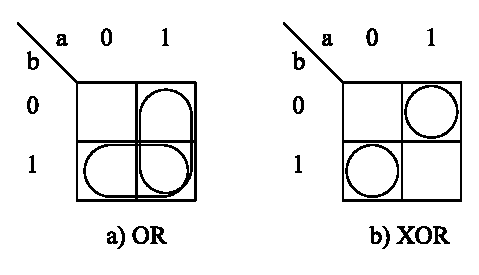
\includegraphics[width=3in]{minterm}
\caption{Satisfying assignments for simple gates}
\label{ORXOR}
\end{figure}

In order to reduce the number of satisfying assignments to be enumerated,
we need \textbf{satisfying assignments minimization} technique to remove irrelevant variables' assignments from satisfying assignment $A$,
so that $A$ can cover more complete satisfying assignments.
For example, for OR gate $z= a\vee b$ in Figure \ref{ORXOR}a),
its complete satisfying assignments that can make $z\equiv 1$ are $\{a= 1, b= 0\}$,$\{a= 1, b= 1\}$ and $\{a= 0, b= 1\}$,
which contain 6 assignments to individual variables.
It's obvious that $\{a= 1, b= 0\}$ and $\{a= 1, b= 1\}$ can be merged into $\{a= 1\}$ by removing $b$.
At the same time,
$\{a= 1, b= 1\}$ and $\{a= 0, b= 1\}$ can also be merged into $\{b= 1\}$ by removing $a$.
Therefore,
these two newly-merged partial assignments contain only two assignments to individual variables,
and are much more succinct than the previous three complete assignments.

Formally,
assume that $\boldsymbol{F}$ is a formula over Boolean variable set $V$,
$\boldsymbol{v}\in V$ is an object variable that should always be 1,
$A$ is a satisfying assignment of $F\wedge v$,
and $U\subseteq V$ is a variable set whose assignments we would like to minimize and enumerate.
We can test whether $u\in U$ is irrelevant to forcing $v$ to 1,
by testing the unsatisfiability of $F\wedge \neg v\wedge A|_{U-\{u\}}$.
If $F\wedge \neg v\wedge A|_{U-\{u\}}$ is unsatisfiable,
then $A|_{U-\{u\}}$ cannot make $v$ to be 0,
so $v$ must still be 1.
Thus,
by removing $u$ from $A$,
we can merge $A$ and $A|_{U-\{u\}}|^{u\to \neg A(u)}$,
and obtain a succinct satisfying assignment $A|_{U-\{u\}}$.

All existing ALLSAT approaches \cite{PRIMECLAUSE,SATUNBMC,MINASS,EFFCON,MINCEX,MEMEFFALLSAT,REPARAM,EFFSATUSMCCO}
share this idea of satisfying assignments minimization.
%To save space,
Here we will present only one of them, i.e., the BFL(brutal force lifting) algorithm \cite{MINASS}:

\vspace{0.2cm}

\begin{algo}
\textbf{$\boldsymbol{ALLSAT}$ based on $\boldsymbol{BFL}$ Algorithm}
\begin{enumerate}%\addtolength{\itemsep}{-0.5\baselineskip}
%{\setlength{\baselineskip}{0.5\baselineskip}
\item $\boldsymbol{ALLSAT}(F,v,U)$ \{
\item \hspace{0.3cm} $SA_v=\{\}$
\item \hspace{0.3cm} while($F\wedge v$ has a satisfying assignment $A$) \{
\item \hspace{0.6cm} $A= \boldsymbol{BFL}(F,v,U,A)$
\item \hspace{0.6cm} $SA_v= SA_v\cup \{A\}$
\item \hspace{0.6cm} $F= F\wedge bcls_A$
\item \hspace{0.3cm} \}
\item \hspace{0.3cm} return $SA_v$
\item \}
\item $\boldsymbol{BFL}(F,v,U,A)$ \{
\item \hspace{0.3cm} foreach $u\in U$
\item \hspace{0.6cm}  if($F\wedge \neg v\wedge A|_{U -\{u\}}$ \textbf{is unsatisfiable})
\item \hspace{0.9cm}     $A= A|_{U -\{u\}}$
%\item \hspace{0.9cm}     $U= U -\{u\}$
%\item \hspace{0.6cm} \}
%\item \hspace{0.3cm} \}
\item \hspace{0.3cm} return $A$
\item \}
\end{enumerate}
\end{algo}

\vspace{0.2cm}

Line 12 will test whether removing $u$ from $A$ can still make $v$ to always take on value 1.
If yes, then $u$ will be removed from both $A$ and $V$.
In this way, $A$ will become a partial assignment covering more complete assignments.

On the other hand,
for XOR gate $z= a \oplus b$ in Figure \ref{ORXOR}b),
its complete satisfying assignments that can make $z\equiv 1$ are $\{a= 1, b= 0\}$ and $\{a= 0, b= 1\}$,
which cannot be merged.
Unfortunately, XOR gates are widely used in almost all communication circuits,
including but not limited to the scrambler and descrambler,
the CRC generator and checker,
the pseudo random test pattern generator and checker.

An extreme example is a $n$-bit comparator that compares two $n$-bit variables.
In this case,
there are $2^n$ complete satisfying assignments,
none of which can be merged with each other.

Thus, enumerating satisfying assignments for XOR intensive circuits is a major difficulty of all existing ALLSAT approaches.
We will solve this problem in Section \ref{sec_buildF}.

%\begin{figure}[tb]
%  \centering
%  \leavevmode
%  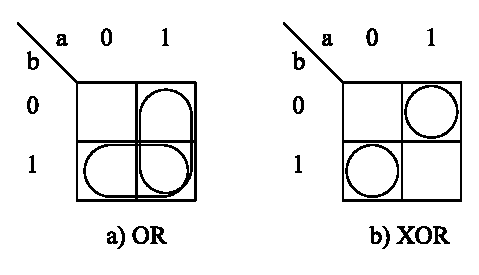
\epsfig{file=minterm.eps}
%\caption{Satisfying assignments for simple gates}
%  \label{ORXOR}
%\end{figure}


\subsection{Checking Reachability with Bounded Model Checking}\label{subsec_bmc}

The description of our algorithm will largely follow that of \textbf{bounded model checking (BMC)} \cite{SMCSAT},
so we present here briefly how to check reachability in BMC.

%\newdef{definition11}{Definition}\label{KripkeStructure}
\vspace{0.2cm}

\begin{definition11}\label{KripkeStructure}
A \textbf{Kripke structure} is a 5-tuple $M=(S,I,T,A,L)$, with a finite set of states $S$,
the set of initial states $I\subseteq S$,
the transition relation between states $T\subseteq S\times S$,
and the labeling of the states $L:S\rightarrow 2^{A}$ with atomic propositions set $A$.
\end{definition11}

\vspace{0.2cm}

BMC is a model-checking technique that considers only limited-length paths.
We call this length the bound of path.
We denote the $i$-th and the $i+1$-th state as $s_i$ and $s_{i+1}$,
and the transition relation between them as $T(s_i,s_{i+1})$.

%We present here only how to check the reachability in BMC,
%and more details can be found in \cite{SMCSAT}.
Let the safety property under verification be $ASSERT$,
the goal of BMC is to find a state that violates $ASSERT$.
Then the BMC problem with bound $b$ can be expressed as:

\begin{equation}\label{bmc}
I(s_0)\wedge \bigwedge_{i=1}^{b-1} T(s_i,s_{i+1})\wedge \bigvee_{i=1}^{b}\neg ASSERT(s_i)
\end{equation}

\begin{figure}[t]
\centering
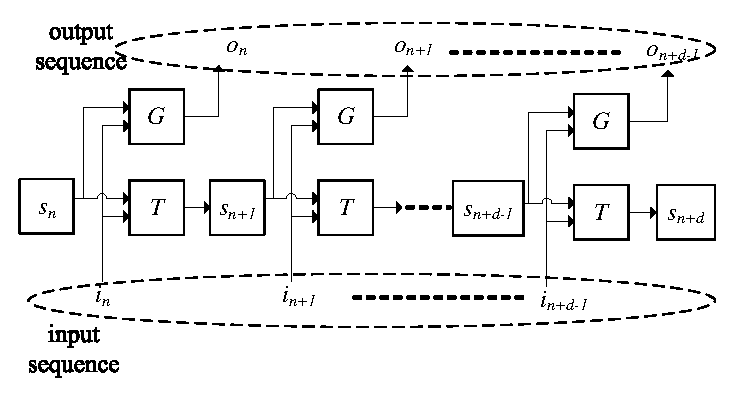
\includegraphics[width=3.5in]{mealy}
\caption{Unfolding Transition Function of Mealy Finite State Machine}
\label{mealyfsm_unfolding}
\end{figure}


We can search for a counterexample of length $b$ by solving Formula \ref{bmc} with a SAT solver.

\section{Checking the Parameterized Complementary Condition}\label{sec_checkUA}

In this section,
we will explain how to check whether the input sequence of circuit $E$ can be recovered from its output sequence.

\subsection{Parameterized Complementary Condition}\label{subsec_pcc}

Our algorithm is concerned about the input and output sequence of circuit $E$,
so \textbf{Mealy finite state machine}\cite{MEALY} is a more suitable model for us than the Kripke structure.

\vspace{0.2cm}

\begin{definition11}\label{MealyFSM}%\addtolength{\itemsep}{-0.5\baselineskip}
%{\setlength{\baselineskip}{0.5\baselineskip}
\textbf{Mealy finite state machine} is a 6-tuple $M=(S,s_0,I,O,T,G)$, consisting of the following
\begin{enumerate}
\item A finite set of states $S$
\item An initial state $s_0\in S$
\item A finite set of letters called the input alphabet $I$
\item A finite set of letters called the output alphabet $O$
\item A state transition function $T: S\times I\to S$
\item An output function $G:S\times I\to O$
\end{enumerate}
%}
\end{definition11}

\vspace{0.2cm}

%\begin{figure*}[tb]
%  \centering
%  \leavevmode
%  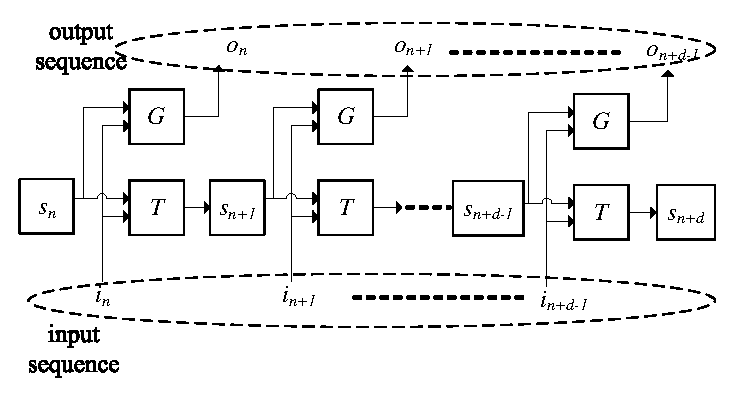
\epsfig{file=mealy.eps}
%\caption{Unfolding Transition Function of Mealy Finite State Machine}
%  \label{mealyfsm_unfolding}
%\end{figure*}

The circuit $E$ can be modeled by such a Mealy finite state machine.
%as shown in Figure \ref{mealyfsm_unfolding}a).
The relationship between its output sequence $o\in O^{\omega}$ and input sequence $i\in I^{\omega}$ is shown in Figure \ref{mealyfsm_unfolding}.
This relationship can be built by unfolding the transition function $T$ and the output function $G$ for $d$ times,
as shown in Formula \ref{unfolding}.

\begin{equation}\label{unfolding}
F_{E}= \bigwedge_{m=n}^{n+d-1} \Big\{ s_{m+1}\equiv T(s_m,i_m) \wedge  o_m\equiv G(s_m,i_m) \Big\}
\end{equation}

In order to recover $i\in I^{\omega}$ from $o\in O^{\omega}$,
we must know how to compute $i_n$ for every $n$,
that is, to find a function $f^{-1}$ that can compute $i_n$ from $o\in O^{\omega}$.

But due to the limited memory of realistic computers,
we cannot take the infinite length sequence $o\in O^{\omega}$ as input to $f^{-1}$.
Instead,
we can only use a finite length sub-sequence of $o$,
which has two parameters,
length $l$ and delay $d$ compared to $i_n$, as shown in Figure \ref{dl}.

\begin{figure}[t]
\centering
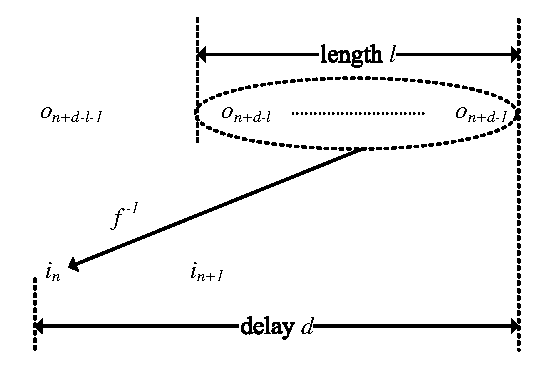
\includegraphics[width=3in]{dl}
\caption{$f^{-1}$ and Parameters of $o$'s Finite Length Subsequence }
\label{dl}
\end{figure}

Thus,
$f^{-1}:O^l\to I$ should be a Boolean function that takes the finite length sequence $<o_{n+d-l},\dots , o_{n+d-1} >$ as its input,
and computes $i_n$.

For a particular pair of $d$ and $l$,
$f^{-1}$ exists if the following condition holds:

\vspace{0.2cm}

\begin{definition11}\label{UniquenessAssumption}
\textbf{Parameterized Complementary Condition}:
For any valuation of the sequence $<o_{n+d-l},\dots , o_{n+d-1} >$,
there exists no more than one valuation of $i_n$
that can make Formula \ref{unfolding} satisfiable.
\end{definition11}

\vspace{0.2cm}
%\begin{figure}[htbp]
%  \centering
%  \leavevmode
%  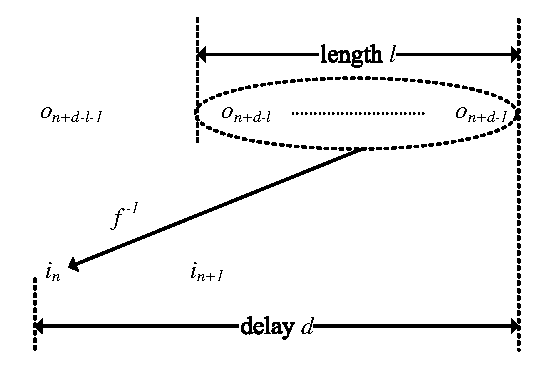
\epsfig{file=dl.eps}
%\caption{$f^{-1}$ and its Parameters}
%  \label{dl}
%\end{figure}

To test whether there exists another $i'_n$ that can make Formula \ref{unfolding} satisfiable,
we need to unfold function $T$ and $G$ for another $d$ times:
\begin{equation}\label{unfolding_again}
F'_{E}= \bigwedge_{m=n}^{n+d-1} \Big\{ s'_{m+1}\equiv T(s'_m,i'_m) \wedge  o'_m\equiv G(s'_m,i'_m) \Big\}
\end{equation}

Obviously,
Formula \ref{unfolding_again} is just another copy of Formula \ref{unfolding},
except that its variables are all renamed by appending a prime.

%Assume that $I_{var}$ and $O_{var}$ are respectively Boolean variable sets that represent $i_n$ and $<o_{n+d-l},\dots , o_{n+d-1} >$,
Thus,
the parameterized complementary condition holds if and only if the following Formula \ref{checkUA} is unsatisfiable.
%\begin{figure}[htbp]
%  \centering
%  \leavevmode
%  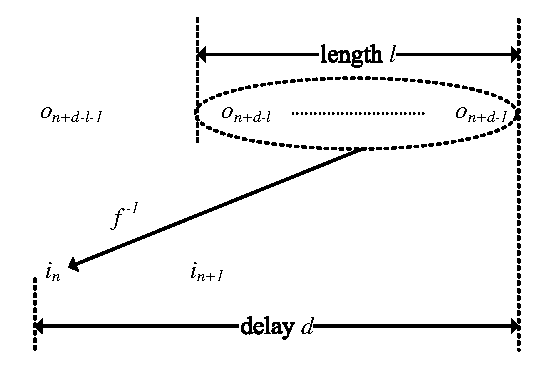
\epsfig{file=dl.eps}
%\caption{$f^{-1}$ and its Parameters}
%  \label{dl}
%\end{figure}
\begin{equation}\label{checkUA}
\begin{array}{c}
%\bigwedge_{m=n}^{n+d-1} \Big\{ s_{m+1}\equiv T(s_m,i_m)\wedge o_m\equiv G(s_m,i_m) \Big\} \wedge \\
%\bigwedge_{m=n}^{n+d-1} \Big\{ s'_{m+1}\equiv T(s'_m,i'_m)\wedge o'_m\equiv G(s'_m,i'_m) \Big\} \wedge \\
F_E \wedge F'_E\wedge \\
\bigwedge_{m=n+d-l}^{n+d-1}o_m\equiv o'_m\wedge \\
i_n\ne i'_n
%\bigwedge_{u\in O_{var}} u\equiv u'\wedge \\
%\bigvee_{v\in I_{var}} v\ne v'
\end{array}
\end{equation}

In Formula \ref{checkUA},
the first line contains two unfolded instances of circuit $E$.
The second line constrains their output sequences $<o_{n+d-l},\dots , o_{n+d-1} >$ and $<o'_{n+d-l},\dots , o'_{n+d-1} >$ to be the same,
and the third line constrains that their input letter $i_n$ and $i'_n$ are different.

For a particular pair of $d$ and $l$ , checking Formula \ref{checkUA} may return two results:
\begin{enumerate}
\item \textbf{Satisfiable}. In this situation,
      for a $<o_{n+d-l},\dots , o_{n+d-1} >$,
      there exists two different $i_n$ and $i'_n$ that can both make Formula \ref{unfolding} satisfiable.
      This means the input letter $i_n$ cannot be uniquely determined by $<o_{n+d-l},\dots , o_{n+d-1} >$.
      %This violates definition \ref{UniquenessAssumption},
      So no $f^{-1}$ exists for this pair of $d$ and $l$.
      We should continue searching for larger $d$ and $l$.
\item \textbf{Unsatisfiable}. In this situation,
      %parameterized complementary condition is satisfied,
      for any valuation of $<o_{n+d-l},\dots , o_{n+d-1} >$,
      there exists no more than one valuation of $i_n$ that can make Formula \ref{unfolding} satisfiable.
      This means the input letter $i_n$ can be uniquely determined by $<o_{n+d-l},\dots , o_{n+d-1} >$.
      So a $f^{-1}$ exists for this pair of $d$ and $l$.
      We will characterize $f^{-1}$ with Formula \ref{unfolding} in Section \ref{sec_buildF}.
\end{enumerate}


\subsection{Ruling out Invalid Input Letters with Assertion}\label{subsec_AST}

Most communication protocols and systems have some restrictions on the valid pattern of input alphabet.
Assume that this restriction is expressed as an assertion predicate $R: I\to \{0,1\}$,
in which $R(i_{n})\equiv 0$ means that $i_n$ is an invalid input letter.
%More formally, assume the set of input Boolean variables is $I_{var}$,
%then $I\subset 2^{I_{var}}$.
Invalid input letters will be mapped to some predefined error output letter,
that is,
for $i_n$,$i'_n\in \{i_m|R(i_m)\equiv 0\}$,
they will both be mapped to the same error output letter $e\in O$.
This will prevent our approach from distinguishing $i_n$ from $i'_n$.

Such restrictions are often documented clearly in the specification of communication protocols.
%and can be found out easily.
Thus,
we choose to employ an assertion-based mechanism,
so that the user can code these restrictions $R$ into their script or source code.

Thus, Formula \ref{unfolding},\ref{unfolding_again} and \ref{checkUA} should be rewritten into the following Formula \ref{unfolding_ast}, \ref{unfolding_again_ast} and \ref{checkUA_ast},
in which the bold formulas are used to account for predicate $R$.

\begin{equation}\label{unfolding_ast}
\begin{split}
\boldsymbol{F_E} &= \\
&
\bigwedge_{m=n}^{n+d-1}
\Big\{
s_{m+1}\equiv T(s_m,i_m) \wedge
o_m\equiv G(s_m,i_m) \wedge
\boldsymbol{R (i_m)}
\Big\}
\end{split}
\end{equation}

\begin{equation}\label{unfolding_again_ast}
\begin{split}
\boldsymbol{F'_E} &= \\
&
\bigwedge_{m=n}^{n+d-1}
\Big\{
s'_{m+1}\equiv T(s'_m,i'_m) \wedge
o'_m\equiv G(s'_m,i'_m) \wedge
\boldsymbol{R (i'_m)}
\Big\}
\end{split}
\end{equation}

\begin{equation}\label{checkUA_ast}
\begin{array}{c}
F_E\wedge F'_E \wedge \\
\bigwedge_{m=n+d-l}^{n+d-1}o_m\equiv o'_m\wedge \\
i_n\ne i'_n
\end{array}
\end{equation}

\subsection{Overapproximating Reachable State Set}\label{subsec_Prfx}
In the previous subsection, we have constrained the valid pattern of $i_m$.
However,
the $s_n$ in Figure \ref{mealyfsm_unfolding} still hasn't been constrained yet.
It may be outside of the reachable state set $RS$ of circuit $E$.
Under some special circumstances,
the parameterized complementary condition may hold on reachable state set $RS$,
but not on unreachable state set.

We can solve this problem by computing the reachable state set $RS$ in Formula \ref{rse},
and constraining that $s_n\in RS$:
%Assume that circuit $E$ can be modeled by Mealy state machine $M_E=(S,s_0,I,O,T,G)$.
%Its reachable state set with assertion predicate $R$ is:

\begin{equation}\label{rse_p_forward}
\begin{split}
RS^{s_0\to p} & =  \Big\{s| \\
& s\equiv s_p\wedge \bigwedge_{m=0}^{p-1}\big\{
s_{m+1}\equiv T(s_m,i_m)\wedge R(i_m)
\big\}\Big\}
\end{split}
\end{equation}

\vspace{0.2cm}

\begin{equation}\label{rse}
RS =\bigcup_{p>0} RS^{s_0\to p}
\end{equation}
%
%Thus, to rule out unreachable $s_n$,
%we need to rewrite Formula \ref{unfolding_ast} and \ref{checkUA_ast}
%into Formula \ref{unfolding_ast_rs} and \ref{checkUA_ast_rs} below:
%
%
%\begin{equation}\label{unfolding_ast_rs}
%\begin{array}{c}
%s_n\in RS \wedge \\
%\bigwedge_{\boldsymbol{m=n}}^{n+d-1}
%\Big\{
%s_{m+1}\equiv T(s_m,i_m) \wedge
%o_m\equiv G(s_m,i_m) \wedge
%R (i_m)
%\Big\}
%\end{array}
%\end{equation}
%
%\begin{equation}\label{checkUA_ast_rs}
%\begin{array}{c}
%s_n\in RS \wedge s'_n\in RS \wedge \\
%\bigwedge_{\boldsymbol{m=n}}^{n+d-1} \Big\{ s_{m+1}\equiv T(s_m,i_m) \wedge o_m\equiv G(s_m,i_m) \wedge R (i_m) \Big\} \wedge \\
%\bigwedge_{\boldsymbol{m=n}}^{n+d-1} \Big\{ s'_{m+1}\equiv T(s'_m,i'_m) \wedge o'_m\equiv G(s'_m,i'_m) \wedge R (i'_m) \Big\} \wedge \\
%\bigwedge_{m=n+d-l}^{n+d-1} o_m\equiv o'_m \wedge \\
%i_n\ne i'_n
%\end{array}
%\end{equation}
%
%%But computing reachable state set $RS$ for large scale circuit $E$ is a very expensive operation that we cannot afford.
%
%Now we have two extreme cases:
%\begin{enumerate}
%\item One extreme case is Formula \ref{unfolding_ast} and \ref{checkUA_ast} with low computation complexity,
%      but high risk of unnecessary fail in checking parameterized complementary condition.
%\item The other extreme case is Formula \ref{unfolding_ast_rs} and \ref{checkUA_ast_rs},
%      which are not affected by unreachable state set,
%      but with very high computation complexity in computing reachable state set $RS$.
%\end{enumerate}
$RS^{s_0\to p}$ in Formula \ref{rse_p_forward} is the set of states that can be reached from the initial state $s_0$ with exact $p$ steps.

%So we need to find a tradeoff between these two extreme cases.
%That should be a method with both acceptable computation complexity and
%low risk of unnecessary fail in checking parameterized complementary condition.

Since it is very expensive to compute $RS$,
%In order to avoid computing $RS$,
we want to overapproximate it with:

\begin{equation}\label{apprse}
\begin{split}
RS^{S\to p} & =  \Big\{s| \\
& s\equiv s_n\wedge \bigwedge_{m=n-p}^{n-1}\big\{
s_{m+1}\equiv T(s_m,i_m)\wedge R(i_m)
\big\}\Big\}
\end{split}
\end{equation}

$RS^{S\to p}$ is the set of states that can be reached within $p$ steps from \textbf{any state} in $S$.
It is obvious that all $RS^{S\to p}$ form a total order relation :
\begin{displaymath}
RS^{S\to p}\subseteq\dots \subseteq RS^{S\to q}\subseteq\dots \textrm{  where } p>q
\end{displaymath}
%
%\begin{figure}[t]
%\centering
%\begin{displaymath}
%\xymatrix{ A \ar[r] & B \ar[d] \\
%D \ar[u] & C \ar[l] }
%\end{displaymath}
%\caption{Counter}
%\label{rmxor}
%\end{figure}

Unfortunately,
$RS$ is not a subset of any $RS^{S\to p}$,
because there may be some state which,
when starting from the initial state,
can only be reached with no more than $p$ steps.
%Unfortunately,
%$RS$ is not a subset of any $RS^{S\to p}$
%because there may exist some state $s\in RS$,
%that when starting from initial state $s_0$,
%can only be reached within $p$ steps,
%and cannot be reached with more than $p$ steps.
For example,
a counter shown below that counts from 0 to 4,
and then stays at 4 forever.
\begin{displaymath}
\begin{array}{cc}
&\curvearrowleft \\
0\to 1\to 2\to 3\to & \underbrace{4}_{RS^{S\to 4}}
\end{array}
\end{displaymath}


In this case,
number 0 to 3 are not in $RS^{S\to p}$,
for $p>3$.

Thus,
we cannot overapproximate $RS$ with $RS^{S\to p}$.

On the other hand,
because circuits $E$ and $E^{-1}$ run in a non-stop way,
we can safely assume that there always exists a prefix state transition sequence with enough length before the current state $s_n$.
Thus,
for any particular $p$,
we only need to consider those states in $\bigcup_{q>p}RS^{s_0\to q}$ instead of $RS$.
Obviously,
$\bigcup_{q>p}RS^{s_0\to q}$ is a subset of $RS^{S\to p}$.
Thus,
we can use $RS^{S\to p}$ as an overapproximation of $\bigcup_{q>p}RS^{s_0\to q}$.

In order to account for $s_n\in RS^{S\to p}$,
we prepend $\bigwedge_{m=n-p}^{n-1}\big\{s_{m+1}\equiv T(s_m,i_m)\wedge R(i_m)\big\}$ to Formula \ref{unfolding_ast},\ref{unfolding_again_ast} and \ref{checkUA_ast},
and obtain Formula \ref{unfolding_ast_p}, \ref{unfolding_again_ast_p} and \ref{checkUA_ast_p}.
Thus,
in addition to parameters $d$ and $l$,
we have a third parameter $p$ to be searched.

\begin{equation}\label{unfolding_ast_p}
\begin{split}
\boldsymbol{F_E} &= \\
&
\bigwedge_{\boldsymbol{m=n-p}}^{n+d-1}
\Big\{
s_{m+1}\equiv T(s_m,i_m) \wedge
o_m\equiv G(s_m,i_m) \wedge
R (i_m)
\Big\}
\end{split}
\end{equation}

\begin{equation}\label{unfolding_again_ast_p}
\begin{split}
\boldsymbol{F'_E} &= \\
&
\bigwedge_{\boldsymbol{m=n-p}}^{n+d-1}
\Big\{
s'_{m+1}\equiv T(s'_m,i'_m) \wedge
o'_m\equiv G(s'_m,i'_m) \wedge
R (i'_m)
\Big\}
\end{split}
\end{equation}

\begin{equation}\label{checkUA_ast_p}
\begin{array}{c}
F_E\wedge F'_E \wedge \\
\bigwedge_{m=n+d-l}^{n+d-1}o_m\equiv o'_m\wedge \\
i_n\ne i'_n
\end{array}
\end{equation}

\textbf{Now putting it all together},
with Formula \ref{unfolding_ast_p}, \ref{unfolding_again_ast_p} and \ref{checkUA_ast_p},
we iterate through all valuations of $d$, $l$ and $p$,
from the smaller one to the larger one,
until we find one valuation of $d$,$l$ and $p$ that makes Formula \ref{checkUA_ast_p} unsatisfiable.
Then $F_E$ in Formula \ref{unfolding_ast_p} will be used in Section \ref{sec_buildF} and \ref{sec_build} to build the complementary circuit $E^{-1}$.

\section{Characterizing $f^{-1}$ with ALLSAT Algorithm Designed for XOR Intensive Circuits}\label{sec_buildF}

If we find the proper values for parameters $d$,$l$ and $p$ in Section \ref{sec_checkUA},
we can now characterize the Boolean function $f^{-1}:O^l\to I$ in this section.

\subsection{Partitioning $f^{-1}$}

According to Section \ref{subsec_Prfx},
the complementary function $f^{-1}:O^l\to I$ is the function that takes $<o_{n+d-l},\dots , o_{n+d-1} >$,
and computes $i_n$ .
It can be characterized from the SAT instance of Formula \ref{unfolding_ast_p}
by enumerating satisfying assignments of $<o_{n+d-l},\dots , o_{n+d-1} >$ and $i_n$.

Assume that $i_n$ is represented by a Boolean variable set $I_{var}$,
and $<o_{n+d-l},\dots , o_{n+d-1} >$ is represented by another Boolean variable set $O_{var}$,
then,
$f^{-1}$ in Boolean domain can be represented as $f^{-1}:\{0,1\}^{O_{var}}\to \{0,1\}^{I_{var}}$,
and can be defined as:

\begin{equation}
f^{-1}= \prod _{v\in I_{var}} f_v^{-1}
\end{equation}

Thus,
characterizing $f^{-1}$ can be partitioned into multiple tasks,
with each task characterizing a Boolean function $f^{-1}_v: \{0,1\}^{O_{var}}\to \{0,1\}$ for a $v\in I_{var}$.
The function $f^{-1}_v$ will be used to compute the value of $v$.

Thus,
in the remainder of this section,
we will focus on characterizing $f^{-1}_v$ instead of $f^{-1}$.

\subsection{Algorithm Framework for Characterizing $f^{-1}_v$}\label{subsec_algframe}
%Assume that the set of all complete satisfying assignments of Formula \ref{unfolding_ast_p} is $\{A_1,\dots ,A_t\}$,
%then $f^{-1}$ can be defined as:
%
%\begin{displaymath}
%\begin{split}
%f^{-1} & (<o_{n+d-l},\dots , o_{n+d-1} >) = \\
%&
%\left\{ \begin{array}{llll}
%A_1(i_n) & & if & \bigwedge_{m=n+d-l}^{n+d-1}o_m\equiv A_1(o_m) \\
%& \dots & & \\
%A_t(i_n) & & if & \bigwedge_{m=n+d-l}^{n+d-1}o_m\equiv A_t(o_m)
%\end{array}
%\right.
%\end{split}
%\end{displaymath}
Assume that $SA_v=\{A_1,\dots,A_m\}$ is the set of satisfying assignments of $F_E\wedge v$,
that is,
the set of satisfying assignments that forces $v$ to 1.
Then $f^{-1}_v$ can be defined as :

\begin{equation}\label{fneg1v}
f^{-1}_v(x) = \left\{ \begin{array}{lll}
1 & & x\equiv A_1(x) \\
  & \dots &  \\
1 & & x\equiv A_m(x) \\
0 & & otherwise
\end{array}
\right.
\end{equation}

But this naive approach suffers from the state space explosion problem.
For $O_{var}$ that contains $k$ Boolean variables,
there may be $2^k$ satisfying assignments in $SA_v$,
which make it impossible to characterize $f^{-1}_v$ for a large $k$.

There exists some much more efficient approaches
to enumerate satisfying assignments of a SAT instance
\cite{PRIMECLAUSE,SATUNBMC,MINASS,EFFCON,MINCEX,MEMEFFALLSAT,REPARAM,EFFSATUSMCCO}.
%including one invented by us\cite{MINCEX}.
According to Subsection \ref{subsec_ALLSAT},
they all try to merge satisfying assignments in $SA_v$ by removing irrelevant variables from each $A\in SA_v$,
so that the size of $SA_v$ can be reduced.

But these approaches are still not efficient enough for our application.
The reasons for their inefficiency and the improvements of our approach are:
\begin{enumerate}
\item XOR gates are used extensively in communication and arithmetic circuits.
As explained in Subsection \ref{subsec_ALLSAT},
the satisfying assignments of XOR cannot be merged by existing approaches.
We solve this problem by discovering XOR gates within $F_E\wedge v$ with $\boldsymbol{XORMIN}$ function.
\item There are lots of redundant clauses in $F_E$.
We use the function $\boldsymbol{SIMPLIFY}$ to simplify $F_E$ to $F_E^v$ before passing it to the main body of $ALLSAT$,
by removing these redundant clauses with unsatisfiable core extraction.
\item The function $BFL$ in Algorithm 1 can remove at most 1 irrelevant variable with each SAT solving. Our improved version $\boldsymbol{BFL\_UNSAT}$ can remove multiple irrelevant variables with every SAT solving. Thus, the number of unnecessary and expensive SAT solving is significantly reduced.
\end{enumerate}

Our new algorithm to characterize $f^{-1}_v$ is presented below.
Its structure is very similar to the function $\boldsymbol{ALLSAT}$ in Algorithm 1,
with our improvements in boldface.

\vspace{0.2cm}

\begin{algo}\label{buildfdec_frm}
\textbf{Characterizing $f^{-1}_v$}
\begin{enumerate}%\addtolength{\itemsep}{-0.5\baselineskip}
%{\setlength{\baselineskip}{0.5\baselineskip}
%\item assume that $\boldsymbol{I_{var}}$ and $\boldsymbol{O_{var}}$ are respectively Boolean variable sets that represent $i_n$ and $<o_{n+d-l},\dots , o_{n+d-1} >$.
%      and $\boldsymbol{F_E}$ is defined in  Formula \ref{unfolding_ast_p}
%\item $G_{XOR}= \{\}$
%\item foreach $v\in I_{var}$ \{
\item \hspace{0.3cm} $\boldsymbol{F_E^v= SIMPLIFY(F_E,v)}$
\item \hspace{0.3cm} $SA_v= \{\}$
\item \hspace{0.3cm} while ( $F_E^v\wedge v$ is satisfiable) \{
\item \hspace{0.6cm} Assume $A$ is a satisfying assignment
\item \hspace{0.6cm} $\boldsymbol{A_{BFL}= BFL\_UNSAT(F_E^v,A,v)}$
%\item \hspace{0.6cm} $\boldsymbol{\{A_{XOR},G\}= XORMIN(F_E^v, A_{BFL},v)}$
\item \hspace{0.6cm} $\boldsymbol{A_{XOR}= XORMIN(F_E^v, A_{BFL},v)}$
\item \hspace{0.6cm} $SA_v= SA_v \cup \{ A_{XOR} \}$
%\item \hspace{0.6cm} $G_{XOR}= G_{XOR}\cup G$
\item \hspace{0.6cm} $F_E^v= F_E^v\wedge bcls_{A_{XOR}}$
%\item \hspace{0.6cm} $F_E^v= F_E^v\wedge \bigwedge _{(x_1= v_1\oplus v_2)\in G}\{x_1\equiv v_1\oplus v_2\}$
\item \hspace{0.3cm} \}
\item \hspace{0.3cm} Characterizing $f^{-1}_v$ as Formula \ref{fneg1v}
%\item \}
%\item $f^{-1}= \prod _{v\in I_{var}} f_v^{-1}$
%}
\end{enumerate}
\end{algo}

\vspace{0.2cm}

%In line 2, $G_{XOR}$ is a set of XOR gates discovered by XORMIN in line 8.
%They will help to speedup the process of enumerating satisfying assignments of $F_E\wedge v\equiv 1$ in line 5.
%More detail will be given in Subsection \ref{subsec_XOR}.
%
%Line 3 will iterate through all input Boolean variables $v\in I_{var}$,
%and characterize a function $f^{-1}_v$ for $v$ in \textbf{line 14},
%$f^{-1}$ can be built from all such $f^{-1}_v$ in \textbf{line 16}.
%The detail of characterizing $f^{-1}_v$ and $f^{-1}$ will be given in Subsection \ref{build_F}.
%
%In line 4,
%$SA_v$ is a set of satisfying assignments that can make $v\equiv 1$,
%this set will be used in line 14 to characterize $f^{-1}_v$.
%
%In line 5,
%we will iterate through all satisfying assignments $A$ of $F_E\wedge v\equiv 1$,
%and minimize them in two steps.
%\begin{enumerate}
%\item \textbf{BFL} in line 7
%is a modified BFL\cite{MINASS} that will be described in Subsection \ref{subsec_BFL}.
%\item \textbf{XORMIN} in line 8 will further minimize the result of BFL by discovering hidden XOR gates,
%and return the minimized assignment $A_{XOR}$ and discovered XOR gate set $G$.
%This is one of our major contributions,
%and will be described in Subsection \ref{subsec_XOR}.
%\end{enumerate}
%
%In line 11,
%we will rule out the enumerated satisfying assignment $A_{XOR}$ by adding its blocking clauses into $F_E$.
%
%In line 12,
%we will add clauses into $F_E$ for newly discovered XOR.

The details of function $SIMPLIFY$, $BFL\_UNSAT$ and $XORMIN$ are described in the following subsections.

\subsection{Simplifying Formula by Extracting Unsatisfiable Core}\label{subsec_sim}
Intuitively,
$F_E$ contains all the clauses necessary to uniquely determine the value of all variables in $I_{var}$.
But when characterizing $f_v^{-1}$ for a particular $v\in I_{var}$,
we only need the set of clauses $F_E^v$ that is necessary to uniquely determine the value of $v$.
This clause set $F_E^v$ must be a subset of $F_E$,
and in most cases,
it is much smaller than $F_E$,
as shown in experimental results.

So we propose the function $\boldsymbol{SIMPLIFY(F_E,v)}$ to simplify $F_E$ to $F_E^v$ for every particular $v$:
\begin{enumerate}
\item The first step is to
extract the unsatisfiable core $F_E^{UNSAT}$ from the following Formula \ref{checkUA_v} with the depth-first approach proposed by Lintao Zhang et al.\cite{VALIDSAT}:
\begin{equation}\label{checkUA_v}
\begin{array}{c}
%\bigwedge_{m=n}^{n+d-1} \Big\{ s_{m+1}\equiv T(s_m,i_m)\wedge o_m\equiv G(s_m,i_m) \Big\} \wedge \\
%\bigwedge_{m=n}^{n+d-1} \Big\{ s'_{m+1}\equiv T(s'_m,i'_m)\wedge o'_m\equiv G(s'_m,i'_m) \Big\} \wedge \\
F_E\wedge F'_E\wedge \\
\bigwedge_{u\in O_{var}} u\equiv u'\wedge \\
v\ne v'
\end{array}
\end{equation}
The unsatisfiability of this formula will be proven in Theorem \ref{thm_checkUA_v} below.
\item The second step is to
intersect the clause set of $F_E$ and $F_E^{UNSAT}$ to get formula $F_E^v$
\begin{equation}\label{checkUA_fev}
F_E^v=F_E\cap F_E^{UNSAT}
\end{equation}
\end{enumerate}

We first need to prove that:
\vspace{0.2cm}
\begin{theorem}[]\label{thm_checkUA_v}
\textbf{Formula \ref{checkUA_v} is unsatisfiable}
\end{theorem}
\begin{IEEEproof}
%Let's prove by contradiction.
%If Formula \ref{checkUA_v} is satisfiable,
%then following Formula \ref{checkUA_rew} is also satisfiable:
%\begin{equation}\label{checkUA_rew}
%\begin{array}{c}
%F_E\wedge F'_E\wedge \\
%\bigwedge_{u\in O_{var}} u\equiv u'\wedge \\
%\bigvee_{v\in I_{var}}v\ne v'
%\end{array}
%\end{equation}
%\vspace{0.2cm}
%
%Because $I_{var}$ is the Boolean variables set that represents input letter $i_n$,
%satisfiable Formula \ref{checkUA_rew} is equivalent to unsatisfiable Formula \ref{checkUA}.
%It is a contradiction,
%so Formula \ref{checkUA_v} must be unsatisfiable.
We can rewrite the unsatisfiable Formula \ref{checkUA_ast_p} by moving $\bigvee_{v\in I_{var}}$ to the outmost layer.
\begin{displaymath}\label{checkUA_rew}
Formula (\ref{checkUA_ast_p})\Rightarrow
\begin{array}{c}
F_E\wedge F'_E\wedge \\
\bigwedge_{u\in O_{var}} u\equiv u'\wedge \\
\bigvee_{v\in I_{var}}v\ne v'
\end{array}
%\Rightarrow
%\begin{array}{c}
%\bigvee_{v\in I_{var}}\Big\{\\
%F_E\wedge F'_E\wedge \\
%\bigwedge_{u\in O_{var}} u\equiv u'\wedge \\
%v\ne v'\Big\}
%\end{array}
\Rightarrow
\begin{array}{c}
\bigvee_{v\in I_{var}}\Big\{\\
Formula (\ref{checkUA_v})\\
\Big\}
\end{array}
\end{displaymath}

%Obviously,
%the formula wrapped in the outmost $\bigvee_{v\in I_{var}}$ is same as Formula \ref{checkUA_v}.
According to this rewritten result,
if for any $v$,
Formula \ref{checkUA_v} is satisfiable,
then the unsatisfiable Formula \ref{checkUA_ast_p} will be satisfiable.
This contradiction concludes the proof.
\end{IEEEproof}

Furthermore,
to replace $F_E$ with $F_E^v$,
we must make sure that $F_E\wedge v$ and $F_E^v\wedge v$ have the same set of satisfying assignments on the variable set $O_{var}$,
which will be enumerated by Algorithm 2.
\begin{theorem}[]\label{thm_fe_fev_eq}
\textbf{$\boldsymbol{F_E\wedge v}$ and $\boldsymbol{F_E^v\wedge v}$ have the same set of satisfying assignments on $\boldsymbol{O_{var}}$}
\end{theorem}
\begin{IEEEproof}
On one hand,
if $A$ is a satisfying assignment of $F_E\wedge v$,
then $A$ is also a satisfying assignment of $F_E^v\wedge v$,
because the clause set of $F_E^v\wedge v$ is a subset of $F_E\wedge v$.

On the other hand,
assume that $A$ is a satisfying assignment of $F_E^v\wedge v$.
%we need to prove that $A$ is also satisfying assignment of $F_E\wedge v$.
%Let's prove by contradiction.
%Assume that $A$ is not satisfying assignment of $F_E\wedge v$,
%According to the definition of $F_E$ in Formula \ref{unfolding_ast_p}, \ref{unfolding_again_ast_p} and \ref{checkUA_ast_p},
%$A|_{O_{var}}$ can force a unique value on $v$:
%\begin{enumerate}
%\item If that value is 1,
%then $F_E\wedge v$ is satisfied.
%This means $A$ is also a satisfying assignment of $F_E\wedge v$.
%\item If that value is 0,
%then $A|_{O_{var}}$ can force $v$ to take a different value on $F_E$ and $F_E^v$.
%This is contradictive to Formula \ref{checkUA_ast_p},
%so value on $v$ cannot be 0.
%\end{enumerate}
According to Formula \ref{checkUA_v} and \ref{checkUA_fev},
the following formula is also unsatisfiable:
\begin{displaymath}
\begin{array}{c}
F_E^v\wedge F'_E\wedge \\
\bigwedge_{u\in O_{var}} u\equiv u'\wedge \\
v\ne v'
\end{array}
\end{displaymath}
because it is a super set of the unsatisfiable core $F_E^{UNSAT}$ of Formula \ref{checkUA_v}.
This formula means that,
no matter what value we assign to $O_{var}$,
we can not make $F_E^v$ and $F_E$ to force different values on $v$.
Thus,
$A$ is also a satisfying assignment of $F_E\wedge v$.

Thus, this theorem is proven.
\end{IEEEproof}

So now,
we can be sure that it is safe to replace $F_E$ with $F_E^v$ to characterize $f^{-1}_v$.
And we will also show in experimental results that such replacing can significantly reduce the size of $F_E$  and run-time overhead.

\subsection{Minimizing Satisfying Assignments by Extracting Unsatisfiable Cores}\label{subsec_bfl}

In Algorithm 1 line 4,
$\boldsymbol{BFL}$ \cite{MINASS} is used to remove those variables irrelevant to forcing $v$ to 1.
%The implementation of $\boldsymbol{BFL}$ has been shown in Algorithm 1.
According to the implementation of $BFL$ in line 11 of Algorithm 1,
every $u\in U$ is tested one by one,
and if the formula in line 12 is unsatisfiable,
$u$ will be removed from $A$.

That is to say,
every unsatisfiability test can remove at most one $u$.
The more $u$ removed,
the more difficult it is to test unsatisfiability.

So the key to reduce the run-time overhead of $BFL$ is to remove more than one $u$ with every unsatisfiability test.
We will achieve this goal through two steps:
\begin{enumerate}
\item In the first step,
computing unsatisfiable core $F^{US}$ of $F\wedge \neg v\wedge A|_{U -\{u\}}$ with the depth-first approach proposed by Lintao Zhang et al.\cite{VALIDSAT}:
\item In the second step,
computing a new $A$ by intersecting the clause set of $A|_{U-\{u\}}$ and $F^{US}$
\end{enumerate}

The implementation of this improved $\boldsymbol{BFL}$ is shown below:
\vspace{0.2cm}
\begin{algo}
\textbf{Improved $\boldsymbol{BFL}$ based on Extracting Unsatisfiable Cores}
\begin{enumerate}
\item $\boldsymbol{BFL\_UNSAT}(F,v,U,A)$ \{
\item \hspace{0.3cm} foreach $u\in U$
\item \hspace{0.6cm}  if($F\wedge \neg v\wedge A|_{U -\{u\}}$ is unsatisfiable) \{
\item \hspace{0.9cm}     \textbf{Assume that $\boldsymbol{F^{US}}$ is unsatisfiable core of $F\wedge \neg v\wedge A|_{U -\{u\}}$}
\item \hspace{0.9cm}     $A= A|_{U -\{u\}}\boldsymbol{\cap F^{US}}$
\item \hspace{0.6cm} \}
\item \hspace{0.3cm} return $A$
\item \}
\end{enumerate}
\end{algo}

Its correctness is proven below:
\vspace{0.2cm}
\begin{theorem}[]\label{thm_BFL_UNSAT}
\textbf{After $\boldsymbol{BFL\_UNSAT}$ is finished, $F\wedge\neg v\wedge A$ is unsatisfiable}
\end{theorem}
\begin{IEEEproof}
We need to prove by induction on the foreach statement in line 2 of Algorithm 3.

For the base case,
according to line 5 of Algorithm 2,
which call $\boldsymbol{BFL\_UNSAT}$,
we know that $A$ is a satisfying assignment of $F_E^v\wedge v$.
Again according to Theorem \ref{thm_checkUA_v} and \ref{thm_fe_fev_eq},
$v$ cannot be 0 under assignment $A$.
So $F\wedge\neg v\wedge A$ is unsatisfiable
when Algorithm 3 reaches the foreach statement in line 2 for the first time.

For the induction step,
assume that when Algorithm 3 reaches the foreach statement in line 2,
$F\wedge\neg v\wedge A$ is unsatisfiable.
Then the if condition in line 3 may be:
\begin{enumerate}
\item \textbf{False}: in this situation,
$A$ will not be changed,
thus $F\wedge\neg v\wedge A$ is still unsatisfiable.

\item \textbf{True}: in this situation,
$F^{US}$ is an unsatisfiable core of $F\wedge\neg v\wedge A|_{U-\{u\}}$,
then $F\wedge\neg v\wedge (A|_{U-\{u\}}\cap F^{US})$ is also unsatisfiable,
because its clause set is a super set of $F^{US}$.
By assigning $A|_{U-\{u\}}\cap F^{US}$ back to $A$ in line 5 of Algorithm 3,
we again get unsatisfiable formula $F\wedge\neg v\wedge A$.
\end{enumerate}

Thus, this theorem is proven.
\end{IEEEproof}

According to theorem \ref{thm_BFL_UNSAT},
$A$ returned by $\boldsymbol{BFL\_UNSAT}$ is also a set of necessary variable assignments that forces $v$ to 1.
Thus $\boldsymbol{BFL}$ can be replaced by $\boldsymbol{BFL\_UNSAT}$ safely.

We will also show in experimental results that
the function $\boldsymbol{BFL\_UNSAT}$ will significantly reduce the number of SAT solving.

\subsection{Minimizing Satisfying Assignments by Discovering XOR Gates}\label{subsec_XOR}

%In order to overcome the problem of BFL,
%we need to discover XOR hidden in result of BFL.
%by checking \textbf{XOR pairing assumption} below.

%\begin{definition11}\label{XORpairingass}
%\textbf{XOR pairing assumption}:
%For a formula $F$ over Boolean variable set $V$,
%a variable $v\in V$ that should always be 1,
%and one satisfying assignments $A_F$ of $F_E\wedge v$,
%assume there is another satisfying assignment $A'_F$,
%such that only two variables $v_1$ and $v_2$ have difference assignment in $A_F$ and $A'_F$ ,
%that is,
%$\{v_i|A_F(v_i)\ne A'_F(v_i)\}\equiv \{v_1,v_2\}$,
%\end{definition11}
%\begin{figure}[b]
%\centering
%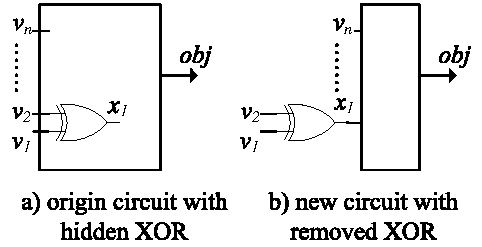
\includegraphics[width=3in]{xor}
%\caption{Discovering Hidden XOR}
%\label{rmxor}
%\end{figure}

According to Algorithm 3,
the assignment $A$ returned by $\boldsymbol{BFL\_UNSAT}$ is a minimal assignment,
which means
removing any variable from $A$ will make it unable to force $v$ to 1.

For $A$ to cover more satisfying assignments,
we need to find a more efficient approach to merge satisfying assignments.

XOR gates are used extensively in communication and arithmetic circuits.
According to Subsection \ref{subsec_ALLSAT} and Figure \ref{ORXOR}b),
the two satisfying assignments of the XOR gate cannot be merged by removing input variables.

But for a larger Boolean function such as $f^{-1}_v$ that \textbf{MAY} contain XOR gate $z=v_1 \oplus v_2$,
we can first check whether this XOR gate actually exists,
and then merge $A$ and $A|_{V-\{v_1,v_2\}}|^{v_1\to \neg A(v_1)}|^{v_2\to \neg A(v_2)}$ by replacing $v_1$ and $v_2$ with $z$ in $A$.

Intuitively,
for a satisfying assignment $A$ that can force $v$ to 1,
assume its domain is $U\subseteq O_{var}$,
for certain $v_1,v_2\in U$,
we can invert the value of $v_1$ and $v_2$ in $A$:

\begin{equation}
A_{\overline{v}_1,\overline{v}_2}=A|_{V-\{v_1,v_2\}}|^{v_1\to \neg A(v_1)}|^{v_2\to \neg A(v_2)}
\end{equation}

We then test whether $A_{\overline{v}_1,\overline{v}_2}$ can also force $v$ to 1,
by checking the unsatisfiability of the following formula:

\begin{equation}\label{check_XPA}
F_E\wedge \neg v\wedge A_{\overline{v}_1,\overline{v}_2}
\end{equation}

%%assume that circuit in Figure \ref{rmxor}a) has an input variable set $V=\{v_1,v_2,v_3,\dots,v_n\}$,
%%and it \textbf{MAY} contain a XOR $v'= v_1\oplus v_2$.
%%We can avoid enumerating the assignments of $v_1$ and $v_2$ %by moving this XOR out of the circuit,
%%%and enumerate assignments of $V\cup\{x_1\}-\{v_1,v_2\}=\{\boldsymbol{x_1},v_3,...,v_n\}$.
%%by first checking the existence of this XOR,
%%and then,
%%as shown in Figure \ref{rmxor}b),
%%if this XOR actually exists,
%%we add another XOR $x_1= v_1\oplus v_2$ into this circuit,
%%and enumerate assignments on $V\cup \{x_1\}-\{v_1,v_2\}$ instead of $V$.
%
%%\begin{figure}[htbp]
%%  \centering
%%  \leavevmode
%%  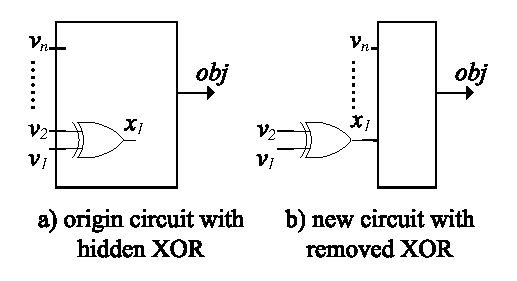
\epsfig{file=xor.eps}
%%\caption{Discovering Hidden XOR}
%%  \label{rmxor}
%%\end{figure}
%
%
%%In order to remove this XOR,
%%we must first make sure that there actually exists a XOR in this circuit.
%
%Formally, to check existence of XOR $v'= v_1\oplus v_2$,
%for a satisfying assignment $A_F$ of formula $F_E\wedge v$,
%we define a new assignment $A_{x_1}$ in Formula \ref{mergeA},
%by first removing assignments of $v_1$ and $v_2$ from $A_F$,
%and then adding assignment of $x_1$ as result of XORing $v_1$ and $v_2$.
%
%\begin{equation}\label{mergeA}
%A_{x_1}= A_F|_{O_{var}-\{v_1,v_2\}}|^{x_1\to A_F(v_1)\oplus A_F(v_2)}
%\end{equation}
%
%With this $A_{x_1}$,
%existence of $v'= v_1\oplus v_2$ can be decided by checking unsatisfiability of the following formula :
%
%\begin{equation}\label{check_XPA}
%F_E\wedge \{x_1\equiv v_1\oplus v_2\}\wedge \neg v\wedge A_{x_1}
%\end{equation}

The unsatisfiability of Formula \ref{check_XPA} means that $A_{\overline{v}_1,\overline{v}_2}$
%just like $A$,
can also force $v$ to 1.

Thus,
$A$ and $A_{\overline{v}_1,\overline{v}_2}$,
which cannot be merged by BFL,
can be merged into:
\begin{equation}\label{mergeA}
A_z= A|_{O_{var}-\{v_1,v_2\}}|^{z\to A(v_1)\oplus A(v_2)}
\end{equation}
with the help of a newly discovered XOR gate that takes $v_1$ and $v_2$ as input,
and output $z$:
\begin{equation}
z=v_1\oplus v_2
\end{equation}

Now,
the support set of $f^{-1}_v$ and $f^{-1}$ will change from $O_{var}$ to $O_{var}\cup \{z\}$.

If we repeatedly check the unsatisfiability of Formula \ref{check_XPA} for other pairs of $v_1$ and $v_2$,
we can discover all hidden XOR gates and merge their satisfying assignments.
All such XOR gates will be used in Subsection \ref{subsec_insxor} to build $E^{-1}$.

%If we repeatedly merge assignments by checking unsatisfiability of Formula \ref{check_XPA},
%we can get a partial assignment of $F_E\wedge \{x_1\equiv\dots\oplus\dots\}\dots\wedge \{x_n\equiv\dots\oplus\dots\}\wedge v$ in Formula \ref{ax1xn},
%which contains $2^n$ complete assignments.
%
%\begin{equation}\label{ax1xn}
%A_{x_1\dots x_n}= A_F|_{O_{var}-\{v_1,\dots\}}|^{x_1\to \dots\oplus\dots}\dots|^{x_n\to \dots\oplus\dots}
%\end{equation}

With the above discussion,
we describe \textbf{XORMIN} below:

\vspace{0.2cm}

\begin{algo}\label{buildfdec}
\textbf{ $\boldsymbol{XORMIN(F_E, A,v)}$}
\begin{enumerate}%\addtolength{\itemsep}{-0.5\baselineskip}
%{\setlength{\baselineskip}{0.5\baselineskip}
\item $G=\{\}$
\item do \{

\item \hspace{0.3cm} $G_{new}=\{\}$  // the set of newly discovered XOR
%\item \hspace{0.3cm} assume the set of variables in $A_F$ is $V$
\item \hspace{0.3cm} foreach $v_1,v_2\in O_{var}$ \{

\item \hspace{0.6cm}   if(\textbf{Formula \ref{check_XPA} is unsatisfiable})\{

\item \hspace{0.9cm}     $G_{new}= G_{new}\cup \{ z= v_1\oplus v_2\}$
\item \hspace{0.9cm}     $A= A|_{O_{var}-\{v_1,v_2\}}|^{z\to A(v_1)\oplus A(v_2)}$
\item \hspace{0.9cm}     $O_{var}= O_{var}\cup \{z\}-\{v_1,v_2\}$
\item \hspace{0.9cm}     $F_E= F_E\wedge bcls_{A}$
\item \hspace{0.9cm}     $F_E= F_E\wedge \bigwedge _{\{z= v_1\oplus v_2\}\in G_{new}}\big\{z\equiv v_1\oplus v_2\big\}$

\item \hspace{0.6cm}   \}
\item \hspace{0.3cm} \}
\item \hspace{0.3cm} $G=G\cup G_{new}$
\item \} while($G_{new}\ne \{\}$)
\item return $A$
%\item return $\{A,G\}$
%}
\end{enumerate}
\end{algo}

\vspace{0.2cm}

In line 1,
$G$ is an empty set that will be used to hold all XOR gates discovered by this algorithm.

In line 2, the do-while statement will repeatedly discover new XOR gates,
until no more XOR gates can be discovered.

In line 4,
the foreach statement will enumerate each pair of $v_1,v_2\in O_{var}$,
and line 5 will test if there is a XOR gate between $v_1$ and $v_2$.

Line 6 will record the newly discovered XOR gate.

Line 7 will compute the newly merged satisfying assignment $A$,
and line 8 will modify the support set of $f^{-1}_v$.
%\vspace{0.2cm}
%\begin{theorem}[]\label{thm_XORMIN}
%\textbf{XORMIN is correct}
%\end{theorem}
%\begin{IEEEproof}
%\end{IEEEproof}

\section{Building Circuit $E^{-1}$ from $f^{-1}$}\label{sec_build}
\begin{figure}[!t]
\centering
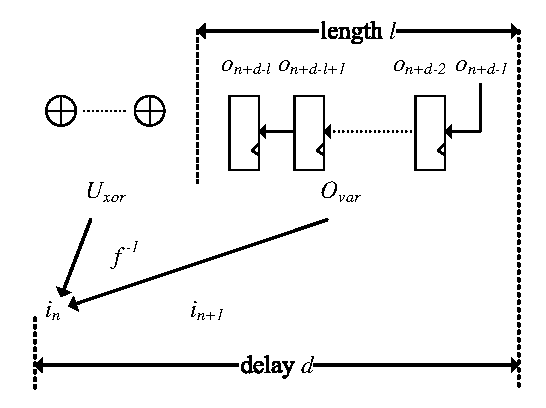
\includegraphics[width=3in]{reg_bank}
\caption{Circuit structure of $E^{-1}$}
\label{reg_bank}
\end{figure}

\subsection{Instantiating Register Bank}
The function $f^{-1}:O^l\to I$ is a Boolean function that takes the finite length sequence $<o_{n+d-l},\dots , o_{n+d-1} >$ as input,
and computes $i_n$.

So while building circuit $E^{-1}$,
as shown in the right-top side of Figure \ref{reg_bank},
we need to instantiate $l-1$ banks of registers to store the subsequence $<o_{n+d-l},\dots , o_{n+d-2} >$,
and connect the output of $o_i$ to the input of $o_{i-1}$.

\subsection{Instantiating Discovered XOR Gates}\label{subsec_insxor}
According to Subsection \ref{subsec_XOR},
assume the set of all XOR gates discovered by function $\boldsymbol{XORMIN}$ is $G$.
Then the output variable set of these XOR gates is:
\begin{equation}
U_{xor}=\Big\{z|\{z=v_1\oplus v_2\}\in G\Big\}
\end{equation}
Then the support set of Boolean function $f^{-1}$ will be changed from $O_{var}$ to $O_{var}\cup U_{xor}$.

So we need to instantiate all XOR gates discovered by the $XORMIN$ function in the generated netlist,
as shown in the left-top side of Figure \ref{reg_bank}.

\subsection{Generating Verilog Source Code for $E^{-1}$}\label{subsec_genverilog}
Assume $SA_v$ is the set of all satisfying assignments that can force $v\in I_{var}$ to 1.
Then the always statement that assigns value to $v$ is shown below:
\begin{enumerate}
\item always@(list of all variables in $O_{var}\cup U_{xor}$) begin
\item \hspace{0.3cm}if($condition_1 || \dots || condition_n$)
\item \hspace{0.6cm} $v<=1'b1$
\item \hspace{0.3cm}else
\item \hspace{0.6cm} $v<=1'b0$
\item end
\end{enumerate}

The $condition_1$ to $condition_n$ in line 2 corresponds to every satisfying assignments in $SA_v$.

\section{Experimental Results}\label{sec_exp}
We implement our algorithm in zchaff\cite{CHAFF},
and run it on a PC with a 2.4GHz AMD Athlon 64 X2 dual core processor, 6GB memory and CentOS 5.2 linux operating system.

All related programs and data files can be downloaded from \url{http://www.ssypub.org}.
\subsection{Benchmarks}
\begin{table}[!t]
\centering
\caption{Information of Benchmarks}
\begin{tabular}{|c|c|c|c|c|c|}
\hline
&XGXS&XFI&scrambler&PCIE&T2 et-\\
&&&&&hernet\\\hline
Line number&&&&&\\
of verilog&214&466&24&1139&1073\\
source code&&&&&\\\hline
\#regs&15&135&58&22&48\\\hline
Data path&8&64&66&10&10\\
width&&&&&\\ \hline
\end{tabular}
\end{table}

%\begin{table}[tb]
%\centering
%\caption{Result of Checking Parameterized Complementary Assumption}
%\begin{tabular}{|c|c|c|c|c|c|}
%\hline
%&XGXS&XFI&scrambler&PCIE&T2 et-\\
%&&&&&hernet\\ \hline
%run time&0.51&71.60&2.51&32.74&44.48\\
%(seconds)&&&&&\\\hline
%$d$      &1       &0     &0         &2   &4          \\ \hline
%$p$      &0       &3     &1         &1   &0          \\ \hline
%$l$      &1       &2     &2         &1   &1          \\ \hline
%\end{tabular}
%\end{table}

%Our approach is the first one that can synthesize complementary circuits automatically,
%so we cannot compare it with other research results.

%Temporal logic synthesis is a research topic that is somewhat close to us,
%but it cannot be scaled to large circuits,
%and no commercial available IP cores are written in temporal logic.
%Thus, it's impossible to compare our result with temporal logic synthesis.

%\begin{table*}[tb]
%\centering
%\caption{Result of Building Complementary Circuits}
%\begin{tabular}{|c|c|c|c|c|c|c|}
%\hline
%       &                 &XGXS&XFI& 66 bit   &PCIE&T2 ethernet	  \\
%       &                 &       &      & scrambler&    &        	  \\ \hline
%BFL    &run time(seconds)&32.67  &$>10,000$&8.56   &$>10,000$&$>10,000$	 	     \\ \cline{2-7}
%only   &line number of   &2927   &N/A   &11882     &N/A &N/A 		     \\
%       &generated verilog&       &      &          &    &        	  \\ \hline
%BFL+   &run time         &1.52   &2939.47&11.97     &47.55&36.64        	  \\ \cline{2-7}
%XORMIN &line number of   &1525   &48829 &4723      &11254& 16616       	  \\
%       &generated verilog&       &      &          &    &        	  \\ \hline
%\end{tabular}
%\end{table*}

Table \Rmnum{1} shows some information of the following benchmarks.
\begin{enumerate}
  \item The first benchmark is a XGXS encoder compliant to clause 48 of IEEE-802.3ae 2002 standard \cite{IEEE80232002}.
  \item The second benchmark is a XFI encoder compliant to clause 49 of the same IEEE standard.
  \item The third benchmark is a 66-bit scrambler used to ensure
that a data sequence has sufficiently many 0-1 transitions
, so that it can run through high-speed
noisy serial transmission channel.
  \item The fourth benchmark is a PCIE physical coding module.
  \item The fifth benchmark is the Ethernet module of Sun's OpenSparc T2 processor.
\end{enumerate}
%\subsection{Result of Checking Parameterized Complementary Condition}

%Table \Rmnum{2} shows the run time of checking parameterized complementary condition on these circuits,
%and the discovered proper values of parameters.

\subsection{Writing Assertions}\label{subsec_writeass}
To write assertions for ruling out invalid input letters,
we refer to the following documentations,
and find out the valid letter patterns easily:
\begin{enumerate}
  \item For the XGXS and T2 ethernet encoders,
  Table 48-2, 48-3 and 48-4 of IEEE-802.3ae 2002 standard \cite{IEEE80232002} describe the pattern of valid letters.
  \item For the XFI encoder and scrambler,
  Figure 49-7 and Table 49-1 of IEEE-802.3ae 2002 standard \cite{IEEE80232002} describe the pattern of valid letters.
  \item For the PCIE physical coding module,
  Table 4-1 of PCI Express Base Specification \cite{PCIESPEC} describe the pattern of valid letters.
\end{enumerate}



\subsection{Result of Checking the Parameterized Complementary Condition}
\begin{table}[!t]
\centering
\caption{Results of Checking the Parameterized Complementary Condition}
\begin{tabular}{|c|c|c|c|c|c|}
\hline
&XGXS&XFI&scra-&PCIE&T2 et-\\
&&&mbler&&hernet\\ \hline
run time&0.51&71.60&2.51&32.74&44.48\\
(seconds)&&&&&\\\hline
$d$      &1       &0     &0         &2   &4          \\ \hline
$p$      &0       &3     &1         &1   &0          \\ \hline
$l$      &1       &2     &2         &1   &1          \\ \hline
\end{tabular}
\end{table}

Table \Rmnum{2} shows the run time of checking the parameterized complementary condition on these circuits,
and the discovered proper values of parameters.

\subsection{Improvement in Run-Time Overhead}
\begin{table}[!t]
\centering
\caption{Run Time of Building Complementary Circuits}
\begin{tabular}{|c|c|c|c|c|c|c|}
\hline
            &&XGXS&XFI& scra-   &PCIE&T2 et-	  \\
            &&       &      & mbler&    &  hernet      	  \\ \hline
BFL    &time(s)&32.67   &time&8.56&time&time 		     \\
only&&&out&&out&out 		     \\ \hline
BFL    &time(s)&1.52   &2939.47&11.97     &47.55&36.64 		     \\ \cline{2-7}
+   &$|F_E|$&25470&5084496&499200&52209&459204\\ \cline{2-7}
XORMIN      &\#SAT&984&137216&8320&528&1032        	  \\ \hline
BFL+     &time(s)&1.08   &752.83 &1.84      &0.82& 27.08       	  \\ \cline{2-7}
XORMIN     &$|F_E^v|$&6694&188717&4807&6635&51204\\ \cline{2-7}
+UNSAT       &\#SAT&480&16828&256&243&538        	  \\ \hline
\end{tabular}
\end{table}
Table \Rmnum{3} compares the following three statistics between the BFL algorithm \cite{MINASS},
BFL+XORMIN proposed in our previous work \cite{ShegnYuShen:iccad09},
and BFL+XORMIN+UNSAT proposed by this paper.
\begin{enumerate}
\item The three \textbf{time} rows compare the run-time overhead of building complementary circuits.
Obviously,
our approach is more than one order of magnitude faster than BFL only approach,
and three times faster than our previous work \cite{ShegnYuShen:iccad09}.
\item $\boldsymbol{|F_E|}$ and $\boldsymbol{|F_E^v|}$ compare the total size of $F_E$ and $F_E^v$ passed to ALLSAT algorithm,
in which $F_E^v$ is the result of simplifying $F_E$ with $\boldsymbol{SIMPLIFY}$.
Obviously,
$\boldsymbol{|F_E^v|}$ is significantly smaller than $\boldsymbol{|F_E|}$.
\item The two \textbf{\#SAT} rows compare the total number of SAT solving invoked by $\boldsymbol{BFL}$ and $\boldsymbol{BFL\_UNSAT}$.
Obviously,
the number of SAT solving is reduced significantly.
\end{enumerate}

\subsection{Comparing Decoder Area}\label{subsec_area}

Table \Rmnum{4} compares the circuit area of hand-written decoders,
decoders built by our previous work\cite{ShegnYuShen:iccad09},
and decoders built by our algorithm.
We synthesize these decoders with LSI10K technology library from Synopsys DesignCompiler.

\begin{table}[!t]
\centering
\caption{Comparing Decoder Area}
\begin{tabular}{|c|c|c|c|c|c|}
\hline
&XGXS&XFI&scrambler&PCIE&T2 et-\\
&&&&&hernet\\ \hline
hand-written      &913       &4886     &1514         &952   &2225          \\
decoders          &&&&&\\ \hline
decoders built     &667       &15269     &1302         &344   &661          \\
by Shen\cite{ShegnYuShen:iccad09}   &&&&&\\ \hline
decoders built     &652       &16659     &1302         &345   &569          \\
by our algorithm   &&&&&\\ \hline
\end{tabular}
\end{table}

From Table \Rmnum{4},
we observe that:
\begin{enumerate}
\item Except for the most complex XFI, our synthesis results
are more compact than hand-written decoders. However,
this comparison is unfair when hand-written decoders
include error-detection and reporting functions, or other
additions not required by the main functionality.
\item For the XFI case,
our circuit area is about 3 times larger than that of hand-written decoders.
This means we need to improve the circuit area in the future work.
\item There is no significant difference in area between our algorithm and our previous work\cite{ShegnYuShen:iccad09}.
\end{enumerate}

\subsection{Comparing Decoder Timing}\label{subsec_timing}
Table \Rmnum{5} compares the critical path latencies of hand-written decoders,
and decoders built by our algorithm.
Their synthesis settings are same as Subsection \ref{subsec_area}.

\begin{table}[!t]
\centering
\caption{Comparing Critical Path Latencies in nanosecond}
\begin{tabular}{|c|c|c|c|c|c|}
\hline
&XGXS&XFI&scrambler&PCIE&T2 et-\\
&&&&&hernet\\ \hline
hand-written      &12.33       &46.65     &6.54         &19.03   &23.36          \\
decoders          &&&&&\\ \hline
decoders built     &13.23       &58.73     &6.54         &8.07   &17.07          \\
by our algorithm   &&&&&\\ \hline
\end{tabular}
\end{table}

According to Table \Rmnum{5},
for most circuits,
the critical path latencies of the decoders built by our algorithm are better than,
or at least close to that of those hand-written decoders.

The only exception is XFI,
the latency of the decoder built by our algorithm is significantly larger than that of hand-written decoder.

One interesting issue that is not shown in Table \Rmnum{5} is,
all these critical paths start from registers, and end at output ports.

\section{Related Works}\label{sec_relwork}
%\subsection{Temporal Logic Synthesis}
%Automatic synthesis of program from logic specification was first identified as Church's problem in 1962\cite{LOGARTHAUTO}.
%Some early researches \cite{SLVSQFSS,AUTOINF} solve this problem by reducing it to checking emptiness of tree automata.
%
%With the invention of temporal logic in the early 1980s,
%this problem had been considered again \cite{DSGSYNTMPLG,SYNTMPLGSPC}.
%But in 1989,
%A. Pnueli and R. Rosner\cite{SYNRCTVMD} pointed out that the complexity of LTL synthesis is double exponent in the size of the formula.
%
%This high complexity drives researchers turning their focus to find smaller but still useful subset of temporal logic,
%such that synthesis problem can be solved with lower complexity.
%
%One line of research \cite{CNTLSYNTMDAUTO,DTMGENGMELTL,SYNRCTVDES} focus on the so-called generalized reactive formulas of the form:
%$(\square \lozenge p_1 \wedge \cdots \square \lozenge p_m) \to (\square \lozenge q_1 \wedge \cdots \square \lozenge q_n)$.
%Complexity of solving synthesis problem for such formula is $O(N^3)$.
%
%The other line of research focus on finding efficient symbolic algorithm \cite{SYNCNTLBNDRPN}
%for expensive safra determination algorithm \cite{CMPLXAUTO} on an useful formula subset,
%or just avoiding it\cite{NEWALGSTRGSYN}.
%
%Based on these research works,
%some tools\cite{ANZU,OPTLTLSYN} that can handle small temporal formulas have been developed.

\subsection{Unsatisfiable Core Extraction}\label{subsec_UNS}


There are many classes of unsatisfiable core extraction algorithms.


The first class of algorithms extract small but not necessary minimal unsatisfiable cores.
Such algorithms are often used to verify the unsatisfiability of certain instance.
Bruni and Sassano\cite{RestoreSat} proposed a constructive approach,
which starts from an initial clause set and iteratively adds new clauses into it,
until the clause set becomes unsatisfiable.
Goldberg and Novikov\cite{VERPROOF} and Zhang and Malik\cite{VALIDSAT} record the resolution graph that generates conflict clauses during a SAT solving,
and trace backward along this graph to find out those clauses that cause the unsatisfiability.
Gershman et al. \cite{DOMINSTOR} tries to find the internal dominator node $d$ in the resolution tree that consumes large number of original clauses, and then tries to prove $d$ without these clauses. When a proof is completed, those clauses can be removed.


The second class of algorithms try to find minimal unsatisfiable cores, whose subsets are all satisfiable.
Oh et al. \cite{AMUSE} adds a clause-selector variable to each clause of the CNF formula, and uses a DPLL-like procedure to find a clause subset with minimal number of clause-selector.
Huang \cite{MUP} also uses the clause-selector variable approach,
but he converts the problem of finding minimal unsatisfiable cores to model counting problem and then uses BDD to solve it.
Dershowitz et al. \cite{ScalableMU} first constructs a resolution graph from the unsatisfiable core,
and then tests every initial clause in this graph to make sure if it is in a minimal core.
Gr\'egoire et al. \cite{LocalMU} uses a local search approach to search for minimal cores.
This approach uses a scoring heuristic that records the common literals between different clauses,
and removes those clauses that aren't likely in a minimal core.
Liffiton and Sakallah\cite{Trim} proposes a preprocessing step to search for
autarkies, which are partial assignments to the variables of a Boolean
CNF formula that satisfy every clause containing an assigned variable.


The third class of algorithms try to find the smallest or minimum cores.
Lynce and Silva\cite{MINIMUM} uses a clause-selector approach similar to AMUSE\cite{AMUSE} mentioned above. It either searches for satisfy and then backtracks to the most recent clause selector variable set to true, or searches for conflicts and then backtracks to a clause selector variable, which means an unsatisfiable core is found.
At this point, it records the size of core and continues searching for smaller cores.
Mneimneh et al. \cite{BranchBoundSMU} and Liffiton et al. \cite{BranchBoundSMUJ} use a branch-and-bound algorithm that utilizes iterative MAXSAT solutions to generate lower and upper bounds on the size of the smallest unsatisfiable core, and branches on specific sub-formulas to find it.
Zhang et al. \cite{GreedyGenetic} uses a greedy genetic algorithm to find the smallest unsatisfiable core.



The fourth class of algorithms try to find out all minimal cores,
so that the complete information about infeasibility can be obtained.
This technique is particularly useful in refining abstract model of model checking.
Bailey and Stuckey\cite{Hitting} and Liffiton and Sakallah \cite{AlgoMUSC} propose to compute minimal unsatisfiable cores
by first computing minimal correction subsets.


\subsection{Satisfying Assignments Enumeration}\label{subsec_relallsat}

The existing ALLSAT algorithms all try to enlarge the complete satisfying assignments,
so that a large state set that contains more complete satisfying assignments can be obtained.

The first approach of this kind is proposed by K. L. McMillan \cite{SATUNBMC}.
He constructs an alternative implication graph in SAT solver,
which records the reasoning relation that leads to the assignment of a particular object variable.
All variables outside this graph can be ruled out from the complete assignment.
Kavita Ravi et al.\cite{MINASS} and P. P. Chauhan et al.\cite{REPARAM} remove those variables whose absence can not make $obj\equiv 0$ satisfiable one by one.
Shen et al.\cite{MINCEX} and HoonSang Jin et al.\cite{PRIMECLAUSE,EFFCON} use an conflict analysis based approach
to remove multiple irrelevant variables in one SAT run.
Orna Grumberg et al.\cite{MEMEFFALLSAT} divides the variable set into an important subset and an unimportant subset.
Variables in the important subset have higher decision priority than those unimportant ones.
Thus,
the important subset formes a search tree,
with each leaf being another search tree for the unimportant set.
%Tobias Nopper et al.\cite{CMPMINCEX} propose an counterexample minimization algorithm for incomplete designs that contain black box.
Cofactoring \cite{EFFSATUSMCCO} qualifies out unimportant variables by setting them to constant value returned by the SAT solver.

\subsection{AND-XOR Logic Synthesis}\label{subsec_XORlogsyn}

The classical logic synthesis works on AND-OR network.
Its core is the two-level logic minimization algorithm,
which aims to find a smaller sum-of-products expression for Boolean function $f$.
%It was obvious that such two-level logic minimization algorithms are very similar to satisfying assignments enumeration described in previous subsection,
%except that they don't work on SAT solvers.

Three best-known two-level logic minimization algorithms are Quine-McCluskey\cite{McCluskey},
Scherzo\cite{Scherzo},
and Espresso-II\cite{Espresso}.

Just like the current ALLSAT that can not deal with XOR-intensive circuits efficiently,
the classical logic synthesis also has the same problem.
Thus,
many researchers propose synthesis algorithms that target XOR-intensive circuits.

One research direction focuses on extending the classical two-level AND-OR minimization to two-level AND-XOR network \cite{Mod2sum,ANDEXOR}.
These works normally describe circuits with the most general ESOP (exclusive sum of product) expressions.
%But extremely high computation complexity of these approaches prevented them from handling large circuits.

Another line of research relies on Reed-Muller expansion\cite{Reed},
and one of its most used variant is Fixed Polarity Reed-Muller Form (FPRM) given by Davio and Deschamps\cite{FPRM},
in which a variable can have either positive or negative polarity.
Some related works that rely on FPRM are \cite{fastexactFPRM,fastOFDD,lowpowerXOR}.

A recent paper\cite{FuncXOR} aims to decompose a function into results of XORing several sub-functions.
So,
this approach can be seen as a generalized form of our XORMIN algorithm,
which discovers XOR between several variables instead of functions.
It is possible that
the circuit area of our generated complementary circuits can be improved by applying this approach to characterize the complementary function $f^{-1}$.


\section{Conclusions and Future Works}\label{sec_con}

In this paper,
we propose a fully automatic approach that synthesizes complementary circuits for communication applications.
According to experimental results,
our approach can synthesize correct complementary circuits for many complex circuits, including but not limited to PCIE and Ethernet.

One direction for future work is to improve the circuit area of generated complementary circuit $E^{-1}$.
According to Section \ref{sec_buildF},
the algorithm XORMIN discovers XOR gates between variables.
It is possible that the same XOR gates can be discovered many times in different iterations.
So if we can decompose the logic formula into multiple functions before applying the XORMIN algorithm,
just like \cite{FuncXOR},
then we can avoid redundant XOR gates and reduce the circuit area.

A recent ICCAD'09 paper by Jiang\cite{IterpoFunc} proposed to use Craig interpolation to characterize a Boolean function from a Boolean relation. We will integrate this algorithm into our framework in the future to reduce the run-time overhead.

%Another possible future work is to automatically generate assertions that rule out invalid input data patterns,
%such that the users can be freed from the burden of inspecting documentation and writing assertions.
Another direction for future work is to deal with circuits with memory array and multiple clocks,
so that more complex communication mechanisms,
such as data link layer and transaction layer,
can be dealt with by our approach.

Yet another direction for future work is to find the termination point for checking the parameterized complementary condition.
We are also considering a debug approach that can find the reason for not terminating within a reasonable time bound.

One issue that isn't addressed by this paper is timing.
The generated complementary circuit has a two-level logic structure.
It seems that the well-known retiming algorithm \cite{Retiming} cannot be applied to such circuits to improve timing.
But we must notice that,
the two-level structure in our generated complementary circuits are built by AND and OR gates with large fanin,
which aren't available in realistic target cell libraries.
When these complementary circuits are mapped to a target cell library with a logic synthesizer,
these large fanin gates will be mapped to a chain of real gates with smaller fanin.
In these mapped circuits,
the retiming algorithm can be applied easily to improve timing.


%\section{todo}
%do experimental result on t2 xpcs and pcie
%
%%prove xormin correct
%
%%modify xormin to factoring XOR
%
%%how to describe parameter p
%
%Example
%
%%implementation detail
%
%draw some figures
%
%say something about size of $F_E$ and $F_E^v$, how they compared
%
%%fix pcie assertion writing
%
%%regenerate $f^{-1}$ figure
%
%%change building $f^{-1}$ to characterization
%
%%compare 3 case: BFL only , BFL+XORMIN , and BFL+XORMIN+UNSAT


% An example of a floating figure using the graphicx package.
% Note that \label must occur AFTER (or within) \caption.
% For figures, \caption should occur after the \includegraphics.
% Note that IEEEtran v1.7 and later has special internal code that
% is designed to preserve the operation of \label within \caption
% even when the captionsoff option is in effect. However, because
% of issues like this, it may be the safest practice to put all your
% \label just after \caption rather than within \caption{}.
%
% Reminder: the "draftcls" or "draftclsnofoot", not "draft", class
% option should be used if it is desired that the figures are to be
% displayed while in draft mode.
%
%\begin{figure}[!t]
%\centering
%\includegraphics[width=2.5in]{myfigure}
% where an .eps filename suffix will be assumed under latex,
% and a .pdf suffix will be assumed for pdflatex; or what has been declared
% via \DeclareGraphicsExtensions.
%\caption{Simulation Results}
%\label{fig_sim}
%\end{figure}

% Note that IEEE typically puts floats only at the top, even when this
% results in a large percentage of a column being occupied by floats.


% An example of a double column floating figure using two subfigures.
% (The subfig.sty package must be loaded for this to work.)
% The subfigure \label commands are set within each subfloat command, the
% \label for the overall figure must come after \caption.
% \hfil must be used as a separator to get equal spacing.
% The subfigure.sty package works much the same way, except \subfigure is
% used instead of \subfloat.
%
%\begin{figure*}[!t]
%\centerline{\subfloat[Case I]\includegraphics[width=2.5in]{subfigcase1}%
%\label{fig_first_case}}
%\hfil
%\subfloat[Case II]{\includegraphics[width=2.5in]{subfigcase2}%
%\label{fig_second_case}}}
%\caption{Simulation results}
%\label{fig_sim}
%\end{figure*}
%
% Note that often IEEE papers with subfigures do not employ subfigure
% captions (using the optional argument to \subfloat), but instead will
% reference/describe all of them (a), (b), etc., within the main caption.


% An example of a floating table. Note that, for IEEE style tables, the
% \caption command should come BEFORE the table. Table text will default to
% \footnotesize as IEEE normally uses this smaller font for tables.
% The \label must come after \caption as always.
%
%\begin{table}[!t]
%% increase table row spacing, adjust to taste
%\renewcommand{\arraystretch}{1.3}
% if using array.sty, it might be a good idea to tweak the value of
% \extrarowheight as needed to properly center the text within the cells
%\caption{An Example of a Table}
%\label{table_example}
%\centering
%% Some packages, such as MDW tools, offer better commands for making tables
%% than the plain LaTeX2e tabular which is used here.
%\begin{tabular}{|c||c|}
%\hline
%One & Two\\
%\hline
%Three & Four\\
%\hline
%\end{tabular}
%\end{table}


% Note that IEEE does not put floats in the very first column - or typically
% anywhere on the first page for that matter. Also, in-text middle ("here")
% positioning is not used. Most IEEE journals use top floats exclusively.
% Note that, LaTeX2e, unlike IEEE journals, places footnotes above bottom
% floats. This can be corrected via the \fnbelowfloat command of the
% stfloats package.



%\section{Conclusion}
%The conclusion goes here.





% if have a single appendix:
%\appendix[Proof of the Zonklar Equations]
% or
%\appendix  % for no appendix heading
% do not use \section anymore after \appendix, only \section*
% is possibly needed

% use appendices with more than one appendix
% then use \section to start each appendix
% you must declare a \section before using any
% \subsection or using \label (\appendices by itself
% starts a section numbered zero.)
%


%\appendices
%\section{Proof of the First Zonklar Equation}
%Appendix one text goes here.

% you can choose not to have a title for an appendix
% if you want by leaving the argument blank
%\section{}
%Appendix two text goes here.


% use section* for acknowledgement
\section*{Acknowledgment}

The authors would like to thank the editors and anonymous reviewers for their hard work.

This work was fund by project 60603088 supported by National Natural Science Foundation of China.

This work was also supported by the Program for Changjiang
Scholars and Innovative Research Team in University No
IRT0614.
% Can use something like this to put references on a page
% by themselves when using endfloat and the captionsoff option.
\ifCLASSOPTIONcaptionsoff
  \newpage
\fi



% trigger a \newpage just before the given reference
% number - used to balance the columns on the last page
% adjust value as needed - may need to be readjusted if
% the document is modified later
%\IEEEtriggeratref{8}
% The "triggered" command can be changed if desired:
%\IEEEtriggercmd{\enlargethispage{-5in}}

% references section

% can use a bibliography generated by BibTeX as a .bbl file
% BibTeX documentation can be easily obtained at:
% http://www.ctan.org/tex-archive/biblio/bibtex/contrib/doc/
% The IEEEtran BibTeX style support page is at:
% http://www.michaelshell.org/tex/ieeetran/bibtex/
%\bibliographystyle{IEEEtran}
% argument is your BibTeX string definitions and bibliography database(s)
%\bibliography{IEEEabrv,tcad10}
%
% <OR> manually copy in the resultant .bbl file
% set second argument of \begin to the number of references
% (used to reserve space for the reference number labels box)
%\begin{thebibliography}{1}
%
%\end{thebibliography}

% Generated by IEEEtran.bst, version: 1.12 (2007/01/11)
\begin{thebibliography}{49}
\providecommand{\url}[1]{#1}
\csname url@samestyle\endcsname
\providecommand{\newblock}{\relax}
\providecommand{\bibinfo}[2]{#2}
\providecommand{\BIBentrySTDinterwordspacing}{\spaceskip=0pt\relax}
\providecommand{\BIBentryALTinterwordstretchfactor}{4}
\providecommand{\BIBentryALTinterwordspacing}{\spaceskip=\fontdimen2\font plus
\BIBentryALTinterwordstretchfactor\fontdimen3\font minus
  \fontdimen4\font\relax}
\providecommand{\BIBforeignlanguage}[2]{{%
\expandafter\ifx\csname l@#1\endcsname\relax
\typeout{** WARNING: IEEEtran.bst: No hyphenation pattern has been}%
\typeout{** loaded for the language `#1'. Using the pattern for}%
\typeout{** the default language instead.}%
\else
\language=\csname l@#1\endcsname
\fi
#2}}
\providecommand{\BIBdecl}{\relax}
\BIBdecl

\bibitem{IEEE80211N}
\BIBentryALTinterwordspacing
C.~Kozup. (2008) Is 802.11n right for you? [Online]. Available:
  \url{http://blogs.cisco.com/wireless/comments/is_80211n_right_for_you/}
\BIBentrySTDinterwordspacing

\bibitem{BRHDVD}
\BIBentryALTinterwordspacing
S.~J. Dubner. (2008) What are the lessons of the blu-ray/hd-dvd battle? a
  freakonomics quorum. [Online]. Available:
  \url{http://freakonomics.blogs.nytimes.com/2008/03/04/what-are-the-lessons-o%
f-the-blu-rayhd-dvd-battle-a-freakonomics-quorum/}
\BIBentrySTDinterwordspacing

\bibitem{CHAFF}
M.~W. Moskewicz, C.~F. Madigan, Y.~Zhao, L.~Zhang, and S.~Malik, ``Chaff:
  Engineering an efficient sat solver,'' in \emph{Proc. {IEEE} International
  Design Automation Conference ({DAC}'01)}, Las Vegas, NV, USA, Jun. 2001, pp.
  530--535.

\bibitem{CoreGen}
\BIBentryALTinterwordspacing
Xilinx. (2008) Xilinx core generator system. [Online]. Available:
  \url{http://www.xilinx.com/tools/coregen.htm}
\BIBentrySTDinterwordspacing

\bibitem{DesignWare}
\BIBentryALTinterwordspacing
Synopsys. (2008) Designware library. [Online]. Available:
  \url{http://www.synopsys.com/IP/DESIGNWARE/Pages/default.aspx}
\BIBentrySTDinterwordspacing

\bibitem{ShegnYuShen:iccad09}
S.~Shen, J.~Zhang, Y.~Qin, and S.~Li, ``Synthesizing complementary circuits
  automatically,'' in \emph{Proc. {IEEE} International Conference on
  Computer-Aided Design ({ICCAD}'09)}, San Jose, California, USA, Nov. 2009,
  pp. 381--388.

\bibitem{BERKMIN}
E.~I. Goldberg and Y.~Novikov, ``Berkmin: A fast and robust sat-solver,'' in
  \emph{Proc. {IEEE} Design, Automation and Test in Europe Conference and
  Exposition ({DATE}'02)}, Paris, France, Mar. 2002, pp. 142--149.

\bibitem{EXTSAT}
N.~E\'en and N.~S\"orensson, ``Extensible sat-solver,'' in \emph{Proc. International Conference on
  Theory and Applications of Satisfiability Testing ({SAT}'03)}, Santa
  Margherita Ligure, Italy, May 2003, pp. 502--518.

\bibitem{VERPROOF}
E.~I. Goldberg and Y.~Novikov, ``Verification of proofs of unsatisfiability for
  cnf formulas,'' in \emph{Proc. {IEEE} Design, Automation and Test in Europe
  Conference and Exposition ({DATE}'03)}, Munich, Germany, Mar. 2003, pp.
  10\,886--10\,891.

\bibitem{VALIDSAT}
L.~Zhang and S.~Malik, ``Validating sat solvers using an independent
  resolution-based checker: Practical implementations and other applications,''
  in \emph{Proc. {IEEE} Design, Automation and Test in Europe Conference and
  Exposition ({DATE}'03)}, Munich, Germany, Mar. 2003, pp. 10\,880--10\,885.

\bibitem{SATLOGICMIN}
S.~Sapra, M.~Theobald, and E.~M. Clarke, ``Sat-based algorithms for logic
  minimization,'' in \emph{Proc. {IEEE} International Conference on Computer
  Design ({ICCD}'03)}, San Jose, CA, USA, Oct. 2003, pp. 510--519.

\bibitem{PRIMECLAUSE}
H.~Jin and F.~Somenzi, ``Prime clauses for fast enumeration of satisfying
  assignments to boolean circuits,'' in \emph{Proc. {IEEE} International Design
  Automation Conference ({DAC}'05)}, San Diego, CA, USA, Jun. 2005, pp.
  750--753.

\bibitem{SATUNBMC}
K.~L. McMillan, ``Applying sat methods in unbounded symbolic model checking,''
  in \emph{Proc. International Conference on Computer Aided Verification
  ({CAV}'02)}, Copenhagen, Denmark, Jul. 2002, pp. 250--264.

\bibitem{MINASS}
K.~Ravi and F.~Somenzi, ``Minimal assignments for bounded model checking,'' in
  \emph{Proc. International Conference on Tools and Algorithms for the
  Construction and Analysis of Systems ({TACAS}'04)}, Barcelona, Spain, Mar.
  2004, pp. 31--45.

\bibitem{EFFCON}
H.~Jin, H.~Han, and F.~Somenzi, ``Efficient conflict analysis for finding all
  satisfying assignments of a boolean circuit,'' in \emph{Proc. International
  Conference on Tools and Algorithms for the Construction and Analysis of
  Systems ({TACAS}'05)}, Edinburgh, UK, Apr. 2005, pp. 287--300.

\bibitem{MINCEX}
S.~Shen, Y.~Qin, and S.~Li, ``Minimizing counterexample with unit core
  extraction and incremental sat,'' in \emph{Proc. International Conference
  Verification, Model Checking, and Abstract Interpretation ({VMCAI}'05)},
  Paris, France, Jan. 2005, pp. 298--312.

\bibitem{MEMEFFALLSAT}
O.~Grumberg, A.~Schuster, and A.~Yadgar, ``Memory efficient all-solutions sat
  solver and its application for reachability analysis,'' in \emph{Proc.
  International Conference Formal Methods in Computer-Aided Design
  ({FMCAD}'04)}, Austin, Texas, USA, Nov. 2004, pp. 275--289.

\bibitem{REPARAM}
P.~Chauhan, E.~M. Clarke, and D.~Kroening, ``A sat-based algorithm for
  reparameterization in symbolic simulation,'' in \emph{Proc. {IEEE}
  International Design Automation Conference ({DAC}'04)}, San Diego, CA, USA,
  Jun. 2004, pp. 524--529.

\bibitem{EFFSATUSMCCO}
M.~K. Ganai, A.~Gupta, and P.~Ashar, ``Efficient sat-based unbounded symbolic
  model checking using circuit cofactoring,'' in \emph{Proc. {IEEE}
  International Conference on Computer-Aided Design ({ICCAD}'04)}, San Jose,
  California, USA, Nov. 2004, pp. 510--517.

\bibitem{SMCSAT}
A.~Biere, A.~Cimatti, E.~M. Clarke, M.~Fujita, and Y.~Zhu, ``Symbolic model
  checking using sat procedures instead of bdds,'' in \emph{Proc. {IEEE}
  International Design Automation Conference ({DAC}'99)}, New Orleans, LA, USA,
  Jun. 1999, pp. 317--320.

\bibitem{MEALY}
M.~G. H, ``A method for synthesizing sequential circuits,'' \emph{Bell Systems
  Technical Journal}, vol.~34, pp. 1045--1079, Jan. 1955.

\bibitem{IEEE80232002}
\emph{IEEE Standard for Information technology Telecommunications and
  information exchange between systems Local and metropolitan area networks
  Specific requirements Part 3: Carrier Sense Multiple Access with Collision
  Detection (CSMA/CD) Access Method and Physical Layer Specifications
  Amendment: Media Access Control (MAC) Parameters, Physical Layers, and
  Management Parameters for 10 Gb/s Operation}, IEEE Std. 802.3, 2002.

\bibitem{PCIESPEC}
\emph{PCI Express Base Specification Revision 2.1}, PCI Special Interest Group
  Std., 2010.

\bibitem{RestoreSat}
R.~Bruni and A.~Sassano, ``Restoring satisfiability or maintaining
  unsatisfiability by finding small unsatisfiable subformulae,''
  \emph{Electronic Notes in Discrete Mathematics}, vol.~9, pp. 162--173, Jun.
  2001.

\bibitem{DOMINSTOR}
R.~Gershman, M.~Koifman, and O.~Strichman, ``Deriving small unsatisfiable cores
  with dominators,'' in \emph{Proc. International Conference Computer Aided
  Verification ({CAV}'06)}, Seattle, WA, USA, Aug. 2006, pp. 109--122.

\bibitem{AMUSE}
Y.~Oh, M.~N. Mneimneh, Z.~S. Andraus, K.~A. Sakallah, and I.~L. Markov,
  ``Amuse: a minimally-unsatisfiable subformula extractor,'' in \emph{Proc.
  {IEEE} International Design Automation Conference ({DAC}'04)}, San Diego, CA,
  USA, Jun. 2004, pp. 518--523.

\bibitem{MUP}
J.~Huang, ``Mup: a minimal unsatisfiability prover,'' in \emph{Proc. {IEEE}
  Conference on Asia South Pacific Design Automation ({ASPDAC}'05)}, Shanghai,
  China, Jan. 2005, pp. 432--437.

\bibitem{ScalableMU}
N.~Dershowitz, Z.~Hanna, and A.~Nadel, ``A scalable algorithm for minimal
  unsatisfiable core extraction,'' in \emph{Proc. International Conference on
  Theory and Applications of Satisfiability Testing ({SAT}'06)}, Seattle, WA,
  USA, Aug. 2006, pp. 36--41.

\bibitem{LocalMU}
\'E.~Gr\'egoire and B.~Mazure and C.~Piette, ``Local-search extraction of muses,'' \emph{Constraints}, vol. 12(3), pp.
  325--344, Sep. 2007.

\bibitem{Trim}
M.~H. Liffiton and K.~A. Sakallah, ``Searching for autarkies to trim
  unsatisfiable clause sets,'' in \emph{Proc. International Conference on
  Theory and Applications of Satisfiability Testing ({SAT}'08)}, Guangzhou,
  China, May 2008, pp. 182--195.

\bibitem{MINIMUM}
I.~Lynce and J.~P.~Marques Silva, ``On computing minimum unsatisfiable cores,'' in \emph{Proc.
  International Conference on Theory and Applications of Satisfiability Testing
  ({SAT}'04)}, Vancouver, BC, Canada, May 2004, pp. 305--310.

\bibitem{BranchBoundSMU}
M.~N.~Mneimneh and I.~Lynce and Z.~S.~Andraus and J.~P.~Marques Silva and K.~A.~Sakallah, ``A branch-and-bound algorithm for extracting smallest minimal
  unsatisfiable formulas,'' in \emph{Proc. International Conference on Theory
  and Applications of Satisfiability Testing ({SAT}'05)}, St. Andrews, UK, Jun.
  2005, pp. 467--474.

\bibitem{BranchBoundSMUJ}
M.~N.~Mneimneh and M.~N.~Mneimneh and I.~Lynce and Z.~S.~Andraus and J.~P.~Marques Silva and K.~A.~Sakallah, ``A branch and bound algorithm for extracting smallest minimal
  unsatisfiable subformulas,'' \emph{Constraints}, vol. 14(4), pp. 415--442,
  Dec. 2009.

\bibitem{GreedyGenetic}
J.~Zhang, S.~Li, and S.~Shen, ``Extracting minimum unsatisfiable cores with a
  greedy genetic algorithm,'' in \emph{Proc. Australian Joint Conference on
  Artificial Intelligence Advances in Artificial Intelligence ({AI}'06)},
  Hobart, Australia, Dec. 2006, pp. 847--856.

\bibitem{Hitting}
J.~Bailey and P.~J. Stuckey, ``Discovery of minimal unsatisfiable subsets of
  constraints using hitting set dualization,'' in \emph{Proc. International
  Symposium Practical Aspects of Declarative Languages ({PADL}'05)}, Long
  Beach, CA, USA, Jan. 2005, pp. 174--186.

\bibitem{AlgoMUSC}
M.~H. Liffiton and K.~A. Sakallah, ``Algorithms for computing minimal
  unsatisfiable subsets of constraints,'' \emph{Journal of Automated Reasoning
  (JAR)}, vol. 40(1), pp. 1--33, Jan. 2008.

\bibitem{McCluskey}
E.~J. McCluskey, \emph{Logic Design Principles}.\hskip 1em plus 0.5em minus
  0.4em\relax Englewood Cliffs, NJ, USA: Prentice-Hall, 1986.

\bibitem{Scherzo}
O.~Coudert, ``On solving covering problems,'' in \emph{Proc. {IEEE}
  International Design Automation Conference ({DAC}'96)}, Las Vegas, Nevada,
  USA, Jun. 1996, pp. 197--202.

\bibitem{Espresso}
R.~L. Rudell and A.~L. Sangiovanni-Vincentelli, ``Multiple-valued minimization
  for pla optimization,'' \emph{IEEE Transactions on CAD}, vol.~6, pp.
  727--750, May 1987.

\bibitem{Mod2sum}
P.~W. Besslich and M.~Riege, ``An efficient program for logic synthesis of
  mod-2 sum expressions,'' in \emph{Proc. ({Euro ASIC}'91)}, Paris, France.

\bibitem{ANDEXOR}
T.~Sasao, ``And-exor expressions and their optimization,'' in \emph{Logic
  Synthesis and Optimization}, T.~Sasao, Ed.\hskip 1em plus 0.5em minus
  0.4em\relax Boston, MA: Kluwer Academic Publishers, 1993.

\bibitem{Reed}
I.~S. Reed, ``A class of multiple-error-correcting codes and their decoding
  scheme,'' \emph{IRE Trans. on Info. Theory}, vol.~6, pp. 48--49, Apr. 1954.

\bibitem{FPRM}
M.~Davio, \emph{Discrete and switching Functions}.\hskip 1em plus 0.5em minus
  0.4em\relax NY: George and McGraw-Hill, 1978.

\bibitem{fastexactFPRM}
A.~Sarabi and M.~A. Perkowski, ``Fast exact and quasi-minimal minimization of
  highly testable fixed-polarity and/xor canonical networks,'' in \emph{Proc.
  {IEEE} International Design Automation Conference ({DAC}'92)}, Anaheim,
  California, USA, Jun. 1992, pp. 30--35.

\bibitem{fastOFDD}
R.~Drechsler, B.~Becker, and M.~Theobald, ``Fast ofdd based minimization of
  fixed polarity reed-muller expressions,'' in \emph{Proc. {IEEE} European
  Design Automation Conference ({EURO-DAC}'94)}, Grenoble, France, Sep. 1994,
  pp. 2--7.

\bibitem{lowpowerXOR}
U.~Narayanan and C.~L. Liu, ``Low power logic synthesis for xor based
  circuits,'' in \emph{Proc. {IEEE} International Conference on Computer-Aided
  Design ({ICCAD}'97)}, San Jose, California, USA, Nov. 1997, pp. 570--574.

\bibitem{FuncXOR}
T.~S. Czajkowski and S.~D. Brown, ``Functionally linear decomposition and
  synthesis of logic circuits for fpgas,'' in \emph{Proc. {IEEE} International
  Design Automation Conference ({DAC}'08)}, Anaheim, CA, USA, Jun. 2008, pp.
  18--23.

\bibitem{IterpoFunc}
J.-H.~R. Jiang, H.-P. Lin, and W.-L. Hung, ``Interpolating functions from large
  boolean relations,'' in \emph{Proc. {IEEE} International Conference on
  Computer-Aided Design ({ICCAD}'09)}, San Jose, California, USA, Jun. 2009,
  pp. 779--784.

\bibitem{Retiming}
C.~E. Leiserson and J.~B. Saxe, ``Optimizing synchronous systems,'' in
  \emph{Proc. {IEEE} Annual Symposium on Foundations of Computer Science
  ({FOCS}'81)}, Nashville, Tennessee, USA, Oct. 1981, pp. 23--36.

\end{thebibliography}


% biography section
%
% If you have an EPS/PDF photo (graphicx package needed) extra braces are
% needed around the contents of the optional argument to biography to prevent
% the LaTeX parser from getting confused when it sees the complicated
% \includegraphics command within an optional argument. (You could create
% your own custom macro containing the \includegraphics command to make things
% simpler here.)
%\begin{biography}[{\includegraphics[width=1in,height=1.25in,clip,keepaspectratio]{mshell}}]{Michael Shell}
% or if you just want to reserve a space for a photo:

%\begin{IEEEbiography}{Michael Shell}
%Biography text here.
%\end{IEEEbiography}

% if you will not have a photo at all:
%\begin{IEEEbiographynophoto}{ShengYu Shen}
\begin{IEEEbiography}[{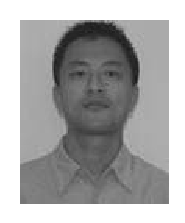
\includegraphics[width=1in,height=1.25in,clip,keepaspectratio]{ssyimg}}]{ShengYu Shen}
(M'10) received the B.S., M.S.
and Ph.D. degrees in computer science from
National University of Defense Technology, ChangSha, HuNan, CHINA in 1997, 2000 and 2005.
He is an Assistant Professor with the School of Computer,
National University of Defense Technology, ChangSha, HuNan, CHINA.
His research
interests are in the areas of formal method with emphasis on counterexample explanation
and logic synthesis.
\end{IEEEbiography}

\begin{IEEEbiography}[{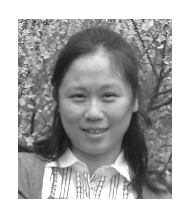
\includegraphics[width=1in,height=1.25in,clip,keepaspectratio]{qyimg}}]{Ying Qin}
 received the B.S. and M.S.
degrees in computer science from
National University of Defense Technology, ChangSha, HuNan, CHINA in 1997 and 2000.
She is an Assistant Professor with the School of Computer,
National University of Defense Technology, ChangSha, HuNan, CHINA.
Her research
interests are in the areas of software engineering with emphasis on operating system implementation.
\end{IEEEbiography}
\newpage
\begin{IEEEbiographynophoto}{KeFei Wang}
received the B.S., M.S.
and Ph.D. degrees in computer science from
National University of Defense Technology, ChangSha, HuNan, CHINA in 1994, 1997 and 2001.
He is an Assistant Professor with the School of Computer,
National University of Defense Technology, ChangSha, HuNan, CHINA.
His research
interests are in the areas of high-performance computing with emphasis on high speed interconnection.
\end{IEEEbiographynophoto}

\begin{IEEEbiographynophoto}{LiQuan Xiao}
received the B.S., M.S.
and Ph.D. degrees in computer science from
National University of Defense Technology, ChangSha, HuNan, CHINA in 1991, 1994 and 1997.
He is an Professor with the School of Computer,
National University of Defense Technology, ChangSha, HuNan, CHINA.
His research
interests are in the areas of high-performance computing with emphasis on high speed interconnection.
\end{IEEEbiographynophoto}

\begin{IEEEbiography}[{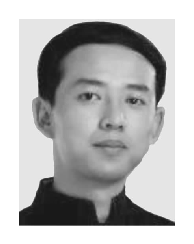
\includegraphics[width=1in,height=1.25in,clip,keepaspectratio]{zjmimg}}]{JianMin Zhang}
received the B.S., M.S.
and Ph.D. degrees in computer science from
National University of Defense Technology, ChangSha, HuNan, CHINA in 2001, 2003 and 2009.
He is an Lecturer with the School of Computer,
National University of Defense Technology, ChangSha, HuNan, CHINA.
His research
interests are in the areas of formal method with emphasis on unsatisfiable core extraction.
\end{IEEEbiography}

\begin{IEEEbiography}[{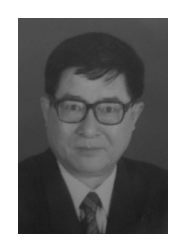
\includegraphics[width=1in,height=1.25in,clip,keepaspectratio]{lskimg}}]{SiKun Li}
received the B.S. degree in computer science from
National University of Defense Technology, ChangSha, HuNan, CHINA in 1968.
He is an Professor with the School of Computer,
National University of Defense Technology, ChangSha, HuNan, CHINA.
His research
interests are in the areas of CAD method for VLSI chips.
\end{IEEEbiography}


% insert where needed to balance the two columns on the last page with
% biographies
%\newpage

%\begin{IEEEbiographynophoto}{Jane Doe}
%Biography text here.
%\end{IEEEbiographynophoto}

% You can push biographies down or up by placing
% a \vfill before or after them. The appropriate
% use of \vfill depends on what kind of text is
% on the last page and whether or not the columns
% are being equalized.

%\vfill

% Can be used to pull up biographies so that the bottom of the last one
% is flush with the other column.
%\enlargethispage{-5in}
%\newpage
%




% that's all folks
\end{document}


